%=======================================================================
%  Pearls AQI Predictor -- Technical Report
%  Compile:  pdflatex aqi_report.tex  (x3, for ToC + refs)
%=======================================================================
\documentclass[11pt,a4paper]{article}

\usepackage[T1]{fontenc}
\usepackage[utf8]{inputenc}
\usepackage{lmodern}
\usepackage[margin=1in]{geometry}
\usepackage{graphicx}
\usepackage{booktabs}
\usepackage{longtable}
\usepackage{array}
\usepackage{multirow}
\usepackage{xspace}
\usepackage[version=4]{mhchem}
\usepackage{amsmath}
\usepackage{amssymb}
\usepackage{siunitx}
\usepackage{caption}
\usepackage{subcaption}
\usepackage{float}
\usepackage{enumitem}
\usepackage{xcolor}
\usepackage{tikz}
\usetikzlibrary{arrows.meta,positioning,shapes.geometric,fit,backgrounds,calc}
\usepackage[hidelinks,breaklinks]{hyperref}
\usepackage{url}

\graphicspath{{../models/}{../data/eda/}{screenshots/}}

\sisetup{detect-all,group-separator={,},group-minimum-digits=4}

% mhchem parses the period in "PM2.5" as an adduct dot, so set it manually.
% \xspace restores the space TeX would otherwise swallow after the macro name.
\newcommand{\pmfine}{PM\textsubscript{2.5}\xspace}

\definecolor{forest}{HTML}{1B5E20}
\definecolor{leaf}{HTML}{43A047}
\definecolor{slate}{HTML}{37474F}
\definecolor{lightbg}{HTML}{ECEFF1}

\captionsetup{font=small,labelfont=bf}

% Thin frame around screenshots, which have light backgrounds at the edges.
\setlength{\fboxsep}{0pt}
\setlength{\fboxrule}{0.4pt}

\title{\vspace{-1.5cm}\textbf{Pearls AQI Predictor}\\[0.35cm]
\large A Serverless End-to-End Machine Learning System for\\
Three-Day Air Quality Index Forecasting}
\author{Ameer Hamza}
\date{6 September 2026}

%=======================================================================
\begin{document}
%=======================================================================

\begin{titlepage}
\centering
\vspace*{2.2cm}

{\Huge\bfseries\color{forest} Pearls AQI Predictor\par}
\vspace{0.6cm}
{\large\itshape A Serverless End-to-End Machine Learning System for\\
Three-Day Air Quality Index Forecasting\par}

\vspace{1.2cm}
\rule{0.75\linewidth}{1.2pt}
\vspace{1.2cm}

{\large\textbf{Ameer Hamza}\par}
\vspace{0.4cm}
{\normalsize Technical Report\par}

\vspace{1.6cm}

\begin{tabular}{@{}r@{\hspace{1.2em}}l@{}}
\textbf{Study area}        & Karachi, Pakistan ($24.8607^\circ$\,N, $67.0011^\circ$\,E)\\[3pt]
\textbf{Forecast horizons} & $+24$\,h, $+48$\,h, $+72$\,h\\[3pt]
\textbf{Feature store}     & \num{8835} hourly observations\\[3pt]
\textbf{Coverage}          & 3 Sep 2025 -- 6 Sep 2026 (368 days)\\[3pt]
\textbf{Deployed model}    & Random Forest (all three horizons)\\[3pt]
\textbf{Repository}        & \url{https://github.com/AmeerHvmza/10pearls_AQI-predictor}\\
\end{tabular}

\vfill
{\large 6 September 2026\par}
\vspace{0.8cm}
\end{titlepage}

%-----------------------------------------------------------------------
\pagenumbering{roman}
\begin{abstract}
\noindent
This report documents the design, implementation and evaluation of the
\emph{Pearls AQI Predictor}, a fully operational machine learning system that
forecasts the United States EPA Air Quality Index for Karachi, Pakistan at
horizons of 24, 48 and 72 hours. The system is deliberately built to be
\emph{100\% serverless}: every scheduled component executes on GitHub Actions
runners, model artefacts and the feature store are versioned in the Git
repository itself, and the user-facing dashboard is hosted on Streamlit
Community Cloud with continuous deployment from the \texttt{main} branch. Air
pollution measurements are obtained from the OpenWeather Air Pollution API and
meteorological variables from the Open-Meteo historical archive; an hourly
pipeline appends fresh observations to a dual-write feature store consisting of
a local Apache Parquet table (the authoritative, dependency-free source of
truth) and a managed Hopsworks feature group populated by stream ingestion. At
the time of writing the store holds \num{8835} consecutive hourly rows spanning
368 days, with no missing measured hours. A nightly training pipeline engineers
64 features, trains four candidate model families -- Ridge regression, Random
Forest, Gradient Boosting and a Keras LSTM -- under five-fold expanding-window
time-series cross-validation, and automatically deploys the best model per
horizon only if it beats a persistence baseline. Random Forest won every
horizon, reducing baseline RMSE by 7.0\%, 10.5\% and 8.1\% at $+24$\,h,
$+48$\,h and $+72$\,h respectively (RMSE 27.43, 34.98, 39.14 AQI points).
Forecasts are explained with SHAP, served with uncertainty bands through a
shared prediction module, and surfaced through both a FastAPI REST interface
and a two-page Streamlit dashboard with EPA-threshold hazard alerting.
\end{abstract}

\vspace{0.5cm}
\tableofcontents
\listoffigures
\listoftables

\clearpage
\pagenumbering{arabic}

%=======================================================================
\section{Introduction}
%=======================================================================

\subsection{Problem Statement}

Ambient air pollution is among the largest environmental risk factors for human
health worldwide. Fine particulate matter (\pmfine) penetrates deep into the
respiratory tract and is causally associated with cardiovascular disease,
respiratory illness, reduced lung function in children, and premature
mortality. South Asian megacities are disproportionately affected, and Karachi
-- the study area for this project -- routinely experiences Air Quality Index
(AQI) values well into the ranges the US Environmental Protection Agency
classifies as \emph{Unhealthy for Sensitive Groups} or worse.

Crucially, the health burden of poor air quality is partially
\emph{avoidable}. Sensitive individuals -- asthmatics, the elderly, young
children, outdoor workers -- can materially reduce their exposure if they know
in advance that a pollution episode is coming: rescheduling outdoor exercise,
using filtration indoors, or wearing appropriate masks. This makes AQI
\emph{forecasting}, as distinct from AQI \emph{monitoring}, a directly
actionable public-health capability. A dashboard that tells a user the air is
already hazardous is informative; one that tells them the air will be hazardous
in two days is useful.

The measured distribution for Karachi over the study period underlines the
point. Across \num{8835} hourly observations the mean AQI is 87.5, but the
series ranges from a minimum of 14.8 to a maximum saturating the 500-point EPA
scale -- an order-of-magnitude swing that an occupant of the city cannot
anticipate without a model.

\subsection{Objectives}

The project was scoped around seven concrete objectives:

\begin{enumerate}[itemsep=2pt]
  \item Build an automated \textbf{feature pipeline} that ingests real air
        pollution and weather observations on an hourly cadence.
  \item \textbf{Backfill} a substantial history of genuine measurements so
        that models can learn seasonal and diurnal structure.
  \item Maintain a \textbf{feature store} that is simultaneously simple enough
        to run with zero external accounts and production-grade enough to
        demonstrate managed-feature-store practice.
  \item Implement a \textbf{training pipeline} that evaluates multiple model
        families per horizon under honest time-series cross-validation and
        automatically promotes the winner to a model registry.
  \item Make every forecast \textbf{explainable} using SHAP.
  \item \textbf{Serve} forecasts through both a machine interface (REST API)
        and a human interface (interactive dashboard), including hazard
        alerting.
  \item Run the whole system on a \textbf{100\% serverless} footing, with no
        manual intervention.
\end{enumerate}

\subsection{The 100\% Serverless Architecture Goal}

A conventional deployment of this system would require at least one always-on
virtual machine to host a scheduler, a database for the feature store, an
object store for model artefacts, and a web server for the front end. That is
four billable components and four things to keep patched.

The architectural thesis of this project is that a system of this class needs
none of them. Instead:

\begin{itemize}[itemsep=2pt]
  \item \textbf{Scheduling} is delegated to GitHub Actions \texttt{cron}
        triggers -- an hourly feature job and a daily training job.
  \item \textbf{The feature store} is an Apache Parquet file committed to the
        repository, giving free versioning, free durability and free
        point-in-time recovery through Git history. A managed Hopsworks
        feature group is written in parallel for production parity.
  \item \textbf{The model registry} is the \texttt{models/} directory in the
        same repository: serialised estimators alongside machine-readable
        metrics and explainability artefacts, all version-controlled.
  \item \textbf{Serving} is a Streamlit Community Cloud application bound
        directly to the repository, rebuilt automatically on every push to
        \texttt{main}.
\end{itemize}

The result is a continuously-updating production ML system with an
infrastructure cost of zero and no server for an operator to log into. The
remainder of this report explains how each layer works and what the system
achieves.

%=======================================================================
\section{System Architecture}
%=======================================================================

The system is organised as a strictly one-directional pipeline: external data
sources feed a feature pipeline, which writes to a feature store, which is read
by both a training pipeline and a serving layer. The training pipeline writes
to a model registry, which the serving layer also reads. Automation drives the
two pipelines on independent schedules. Figure~\ref{fig:arch} shows the
complete data flow.

\begin{figure}[H]
\centering
\resizebox{\textwidth}{!}{%
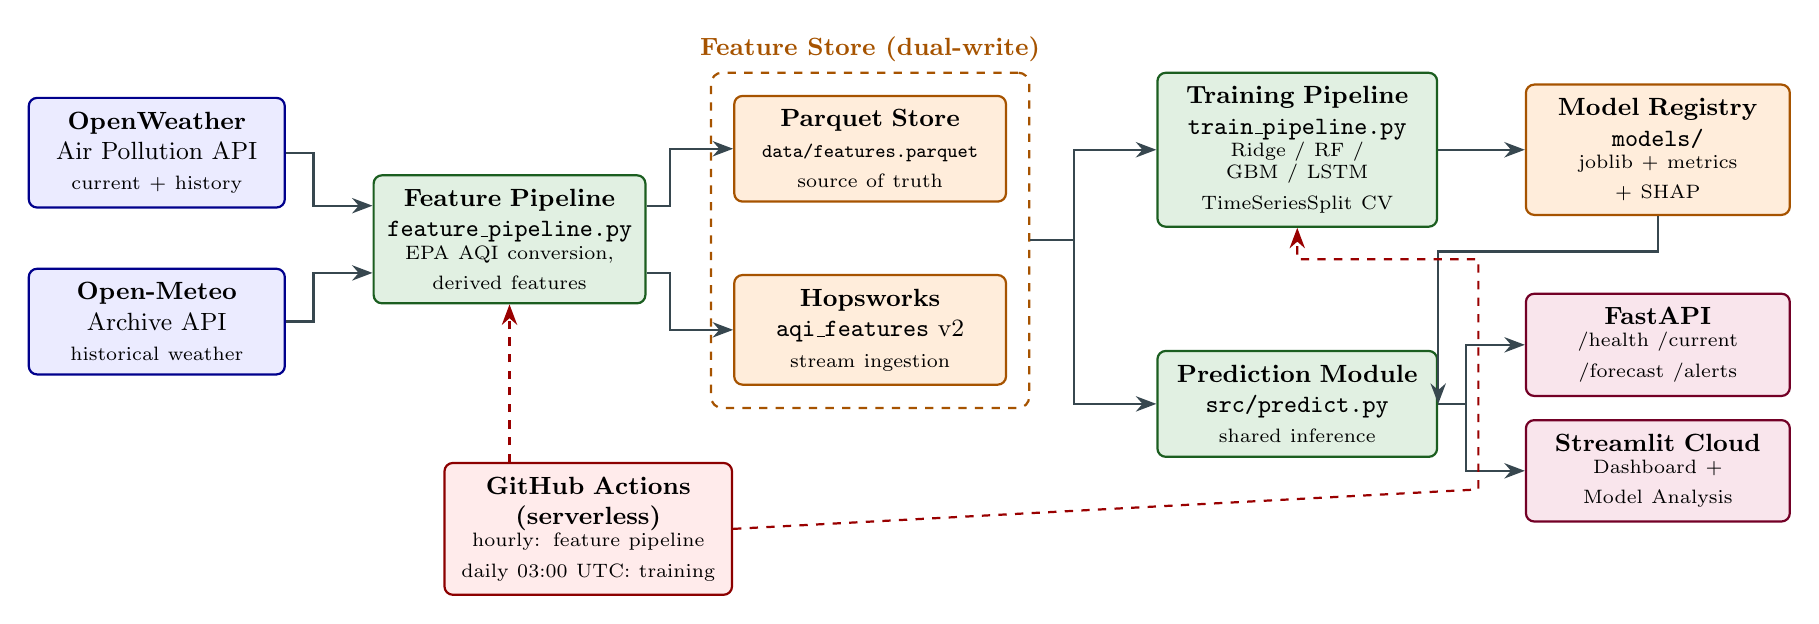
\begin{tikzpicture}[
  font=\small,
  node distance=0.75cm and 1.1cm,
  box/.style={draw=slate,thick,rounded corners=3pt,fill=lightbg,
              align=center,minimum height=1.0cm,inner sep=5pt,text width=2.9cm},
  src/.style={box,fill=blue!8,draw=blue!55!black},
  proc/.style={box,fill=leaf!16,draw=forest},
  store/.style={box,fill=orange!14,draw=orange!65!black},
  serve/.style={box,fill=purple!10,draw=purple!60!black},
  auto/.style={box,fill=red!8,draw=red!55!black,text width=3.3cm},
  ar/.style={-{Stealth[length=2.6mm]},thick,draw=slate},
  sched/.style={ar,dashed,draw=red!60!black},
]

% ---- Sources
\node[src] (ow)  {\textbf{OpenWeather}\\Air Pollution API\\{\scriptsize current + history}};
\node[src,below=of ow] (om) {\textbf{Open-Meteo}\\Archive API\\{\scriptsize historical weather}};

% ---- Feature pipeline
\node[proc,right=of ow,yshift=-1.1cm,text width=3.1cm] (fp)
     {\textbf{Feature Pipeline}\\\texttt{feature\_pipeline.py}\\{\scriptsize EPA AQI conversion,\\derived features}};

% ---- Feature store (dual)
\node[store,right=of fp,yshift=1.15cm,text width=3.1cm] (pq)
     {\textbf{Parquet Store}\\{\scriptsize\texttt{data/features.parquet}}\\{\scriptsize source of truth}};
\node[store,right=of fp,yshift=-1.15cm,text width=3.1cm] (hw)
     {\textbf{Hopsworks}\\\texttt{aqi\_features} v2\\{\scriptsize stream ingestion}};
\node[draw=orange!65!black,thick,dashed,rounded corners=4pt,
      fit=(pq)(hw),inner sep=8pt,label={[orange!65!black]above:\textbf{Feature Store (dual-write)}}] (fsbox) {};

% ---- Training
\node[proc,right=1.6cm of fsbox.east,yshift=1.15cm,text width=3.2cm] (tr)
     {\textbf{Training Pipeline}\\\texttt{train\_pipeline.py}\\{\scriptsize Ridge / RF / GBM / LSTM\\TimeSeriesSplit CV}};
\node[store,right=of tr,text width=3.0cm] (reg)
     {\textbf{Model Registry}\\\texttt{models/}\\{\scriptsize joblib + metrics\\+ SHAP}};

% ---- Serving
\node[proc,below=1.55cm of tr,text width=3.2cm] (pr)
     {\textbf{Prediction Module}\\\texttt{src/predict.py}\\{\scriptsize shared inference}};
\node[serve,right=of pr,yshift=0.75cm,text width=3.0cm] (api)
     {\textbf{FastAPI}\\{\scriptsize /health /current\\/forecast /alerts}};
\node[serve,right=of pr,yshift=-0.85cm,text width=3.0cm] (st)
     {\textbf{Streamlit Cloud}\\{\scriptsize Dashboard +\\Model Analysis}};

% ---- Arrows
\draw[ar] (ow.east) -- ++(0.35,0) |- ([yshift=-4mm]fp.north west);
\draw[ar] (om.east) -- ++(0.35,0) |- ([yshift=4mm]fp.south west);
\draw[ar] ([yshift=-4mm]fp.north east) -- ++(0.3,0) |- (pq.west);
\draw[ar] ([yshift=4mm]fp.south east)  -- ++(0.3,0) |- (hw.west);
\draw[ar] (fsbox.east) -- ++(0.55,0) |- (tr.west);
\draw[ar] (fsbox.east) -- ++(0.55,0) |- (pr.west);
\draw[ar] (tr.east)   -- (reg.west);
\draw[ar] (reg.south) -- ++(0,-0.45) -| (pr.east);
\draw[ar] (pr.east) -- ++(0.35,0) |- (api.west);
\draw[ar] (pr.east) -- ++(0.35,0) |- (st.west);

% ---- Automation band
\node[auto,below=2.0cm of fp.south,xshift=1.0cm] (gha)
     {\textbf{GitHub Actions (serverless)}\\{\scriptsize hourly: feature pipeline\\daily 03:00 UTC: training}};
\draw[sched] (gha.north -| fp.south) -- (fp.south);
\draw[sched] (gha.east) -- ($(pr.south)+(2.3,-0.4)$)
                        -- ($(tr.south)+(2.3,-0.4)$)
                        -- ($(tr.south)+(0,-0.4)$) -- (tr.south);

\end{tikzpicture}}
\caption[System architecture]{End-to-end architecture of the Pearls AQI
Predictor. Solid arrows are data flow; dashed red arrows are scheduled
invocation by GitHub Actions. The feature store is written twice (local
Parquet plus a managed Hopsworks feature group) but read once, from Parquet.
Both serving surfaces share a single prediction module, so the REST API and
the dashboard cannot disagree.}
\label{fig:arch}
\end{figure}

\subsection{Layer Responsibilities}

\begin{description}[leftmargin=0pt,style=nextline,itemsep=3pt]
  \item[Ingestion layer.] Two external providers are used for complementary
    reasons. OpenWeather supplies pollutant concentrations both in real time
    and as a queryable history back to late 2020, under a single free-tier
    key. Open-Meteo supplies the historical meteorological archive without
    requiring a key at all. The feature pipeline converts raw pollutant
    concentrations into a US EPA AQI value before anything downstream sees
    them.
  \item[Feature store layer.] A single Parquet table on a continuous hourly
    grid, keyed by UTC \texttt{timestamp}. Every writer goes through
    \texttt{utils.save\_feature\_store}, which merges, de-duplicates on
    timestamp, and then attempts the Hopsworks dual-write.
  \item[Training layer.] Reads the whole store, engineers features, runs
    cross-validated model selection per horizon, and writes exactly three
    artefact sets to the registry -- one per horizon.
  \item[Registry layer.] Plain files: \texttt{model\_\{h\}h.joblib} bundles
    (estimator, fitted scaler, feature column list, residual statistics,
    baseline verdict), \texttt{metrics\_\{h\}h.json}, and the SHAP outputs.
    Because these are committed to Git, every retrain is an auditable diff.
  \item[Serving layer.] \texttt{src/predict.py} is the only code path that
    turns a feature store row into a forecast. FastAPI and Streamlit are both
    thin presentation wrappers over it.
  \item[Automation layer.] Two GitHub Actions workflows sharing a
    \texttt{concurrency} group, so the hourly and daily jobs can never
    collide when they both attempt to commit at 03:00 UTC.
\end{description}

%=======================================================================
\section{Data Pipeline}
%=======================================================================

\subsection{How Data Is Collected}

Data acquisition is split into a one-off historical backfill and a recurring
hourly increment.

\paragraph{Historical backfill (\texttt{src/backfill.py}).}
Pollutant history is requested from the OpenWeather air-pollution history
endpoint,
\texttt{api.openweathermap.org/data/2.5/air\_pollution/history}, in
30-day chunks to stay inside the endpoint's per-request window. Weather history
for the same interval is requested from the Open-Meteo archive,
\texttt{archive-api.open-meteo.com/v1/archive}, which needs no API key. The two
responses are joined on the UTC hour. Every backfill run is recorded in
\texttt{data/PROVENANCE.md} together with the exact command, the number of
successful HTTP 200 responses, the number of records returned by each provider,
the number of rows actually written, and a SHA-256 checksum of the resulting
Parquet file. The first raw JSON response from each provider is retained
verbatim in \texttt{data/provenance\_first\_pollution.json} and
\texttt{data/provenance\_first\_weather.json} as physical evidence that the
history is measured rather than synthesised.

\paragraph{Hourly increment (\texttt{src/feature\_pipeline.py}).}
Once per hour a GitHub Actions runner executes the feature pipeline, which
fetches the current pollutant concentrations and current weather for the
configured coordinates, converts them to an AQI, assembles a single feature
row, and merges it into the store. The merge is idempotent: rows are
de-duplicated on \texttt{timestamp}, so a re-run of the same hour updates
rather than duplicates.

\paragraph{AQI computation.}
The AQI is not taken from the provider's own 1--5 index. Instead
\texttt{owm\_aqi\_to\_us\_aqi()} implements the EPA definition directly: the
AQI is the \emph{maximum} of the per-pollutant sub-indices computed over
\pmfine, \ce{PM10}, \ce{O3}, \ce{CO}, \ce{SO2} and \ce{NO2}. Gaseous species
are converted from \si{\micro\gram\per\cubic\metre} to ppb or ppm at
\SI{25}{\celsius} and \SI{1}{atm} before breakpoint lookup, and each
concentration is truncated to its breakpoint table's published precision --
without truncation a \pmfine reading of \SI{12.03}{\micro\gram\per\cubic\metre}
falls in the gap between the 12.0 and 12.1 breakpoints and matches no bucket.
Because concentrations are stored raw, the AQI column can be recomputed at any
time by \texttt{src/repair\_feature\_store.py} if the conversion is refined.

\subsection{Final Dataset}

Table~\ref{tab:dataset} summarises the feature store as it stands.

\begin{table}[H]
\centering
\caption{Feature store characteristics (\texttt{data/features.parquet}).}
\label{tab:dataset}
\small
\begin{tabular}{@{}lr@{}}
\toprule
\textbf{Property} & \textbf{Value}\\
\midrule
Location & Karachi ($24.8607^\circ$\,N, $67.0011^\circ$\,E)\\
Hourly rows & \num{8835}\\
Rows with a measured AQI & \num{8835} (100\%)\\
Imputed rows & 0\\
Stored columns & 27\\
Start of coverage (UTC) & 2025-09-03 00:00\\
End of coverage (UTC) & 2026-09-06 02:00\\
Span & 368 days\\
Maximum inter-observation gap & \SI{1}{hour}\\
Mean AQI & 87.52\\
Minimum / maximum AQI & 14.8 / 500.0\\
Mean \pmfine & \SI{31.90}{\micro\gram\per\cubic\metre}\\
File size & \SI{504596}{byte}\\
\bottomrule
\end{tabular}
\end{table}

The store was assembled incrementally, and \texttt{data/PROVENANCE.md} records
each stage: an initial 90-day backfill yielding \num{2055} rows
(2026-06-03 to 2026-08-27), a subsequent 365-day pull merged to \num{8761}
rows, and a consolidation and AQI-recomputation pass producing the unified
\num{8825}-row store with zero measured hours lost. The hourly pipeline has
carried it forward from there to the current \num{8835} rows.

\paragraph{Raw columns.} The stored schema comprises the UTC
\texttt{timestamp}; eight pollutant concentrations (\texttt{co}, \texttt{no},
\texttt{no2}, \texttt{o3}, \texttt{so2}, \texttt{pm2\_5}, \texttt{pm10},
\texttt{nh3}); six meteorological variables (\texttt{temp}, \texttt{humidity},
\texttt{pressure}, \texttt{wind\_speed}, \texttt{wind\_deg}, \texttt{clouds});
calendar fields; the computed \texttt{aqi} and provider \texttt{aqi\_raw}; an
\texttt{is\_imputed} flag; and three lightweight derived columns persisted at
ingestion time.

\subsection{Feature Engineering}

Persisting only raw observations keeps the store small and re-derivable;
the full feature set is constructed on demand by
\texttt{train\_pipeline.engineer\_features()}, which is called identically at
training time and at inference time. This shared function is the single
guarantee against train/serve skew. It expands the 27 stored columns into
\textbf{64 model features} in six groups.

\begin{table}[H]
\centering
\caption{Engineered feature groups.}
\label{tab:features}
\small
\renewcommand{\arraystretch}{1.25}
\begin{tabular}{@{}p{3.5cm}p{4.0cm}p{6.6cm}@{}}
\toprule
\textbf{Group} & \textbf{Construction} & \textbf{Rationale}\\
\midrule
Cyclical time &
$\sin,\cos$ of hour, day-of-week and month &
Hour 23 and hour 0 are adjacent in reality but maximally distant as integers;
sine/cosine pairs restore that adjacency. Karachi shows a strong diurnal
pollution cycle.\\

AQI lags &
$t-1,2,3,6,12,24,48$\,h &
Air quality is highly autocorrelated. The 24\,h and 48\,h lags additionally
encode same-time-yesterday behaviour.\\

Rolling statistics &
mean, standard deviation, minimum, maximum over $3,6,12,24$\,h windows &
The mean gives a denoised level, the standard deviation gives local
volatility, and min/max bracket the recent envelope.\\

Rates of change &
first differences at $1,3,6,24$\,h; deviation of current AQI from its 6\,h and
24\,h rolling means &
Distinguishes a rising episode from a falling one at the same absolute level --
the same AQI means very different things on the way up and on the way down.\\

Pollutant and weather lags &
\pmfine at $1,3,6,24$\,h; wind speed and humidity at $6,24$\,h &
\pmfine is the dominant AQI driver locally; yesterday's wind and humidity
condition today's accumulation.\\

Interactions &
$\text{wind speed}\times\pmfine$;
$\text{temp}\times\text{humidity}$;
6\,h pressure difference &
Encodes dispersal (wind clears particulates), inversion conditions (warm and
humid air traps pollution), and frontal passage.\\
\bottomrule
\end{tabular}
\end{table}

Two further design decisions in this stage are worth stating explicitly.

First, all lag and rolling operations are \emph{positional} (\texttt{shift},
\texttt{rolling}), which is only correct on an unbroken hourly index. The store
is therefore always passed through \texttt{utils.to\_hourly\_grid()} before
feature construction, so that \texttt{shift(24)} genuinely means ``24 hours
ago'' and not ``24 records ago''.

Second, AQI values above the 99th percentile are capped before lag and rolling
features are derived. Karachi's series contains short extreme spikes that
otherwise propagate through 24 hours of rolling windows and dominate the fit.

\subsection{Exploratory Data Analysis}

\texttt{notebooks/eda.py} regenerates three diagnostic figures from the live
store (Figure~\ref{fig:eda}). They establish the three properties the feature
design relies on: a strong diurnal cycle, dominance of particulate matter over
gaseous pollutants, and heavy autocorrelation with episodic spikes.

\begin{figure}[H]
\centering
\begin{subfigure}[t]{0.48\textwidth}
  \centering
  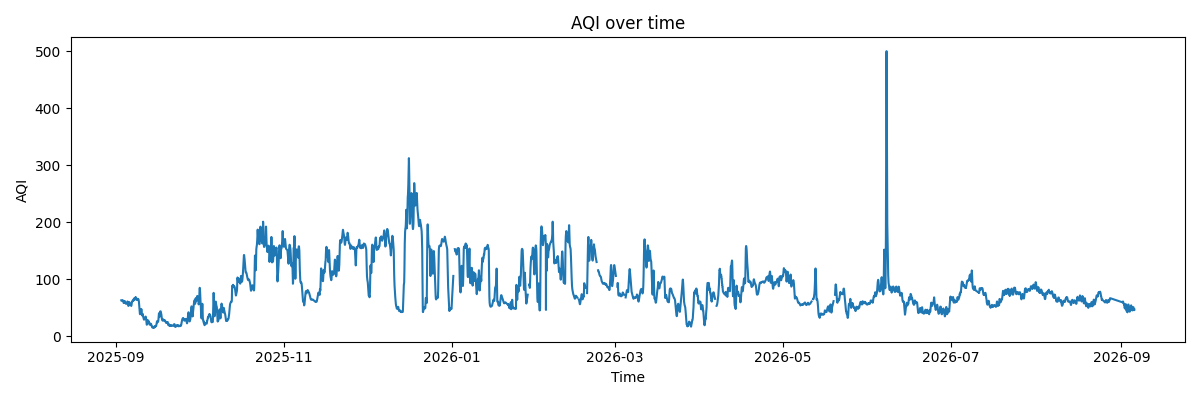
\includegraphics[width=\linewidth]{aqi_timeseries.png}
  \caption{AQI over the full coverage period.}
\end{subfigure}\hfill
\begin{subfigure}[t]{0.48\textwidth}
  \centering
  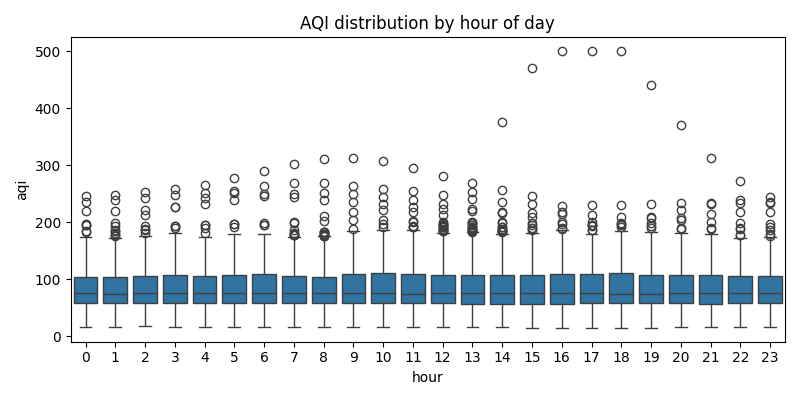
\includegraphics[width=\linewidth]{aqi_by_hour.png}
  \caption{AQI distribution by hour of day.}
\end{subfigure}

\vspace{0.5cm}
\begin{subfigure}[t]{0.62\textwidth}
  \centering
  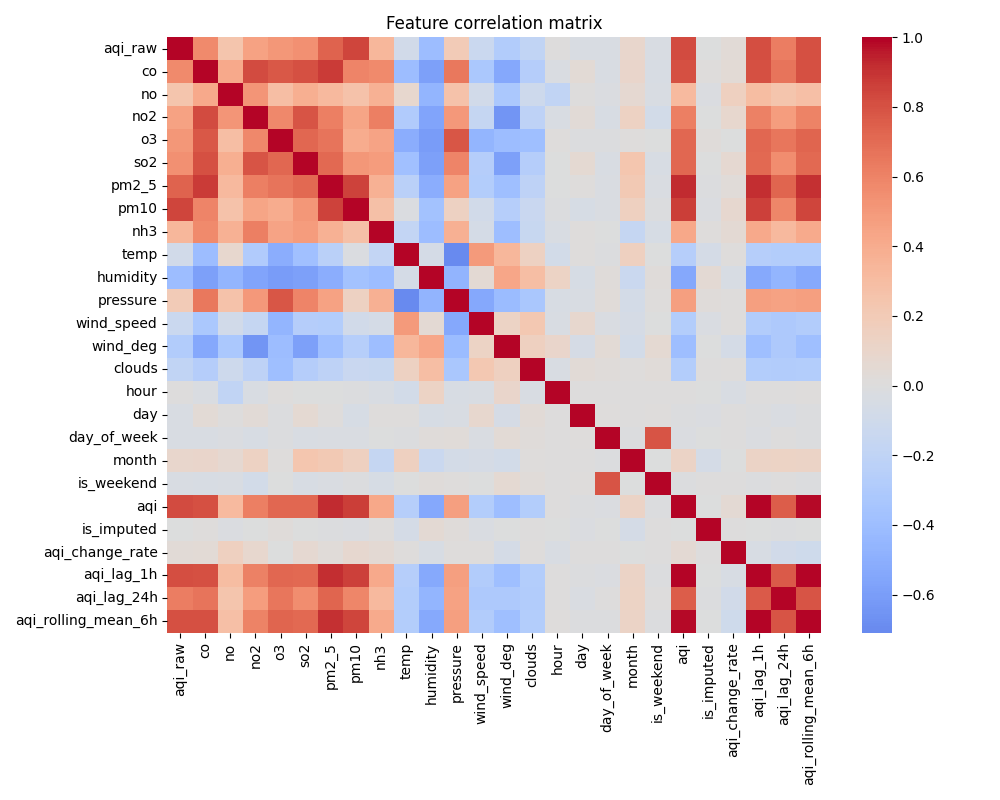
\includegraphics[width=\linewidth]{correlation_heatmap.png}
  \caption{Correlation matrix of numeric features.}
\end{subfigure}
\caption[Exploratory data analysis]{Exploratory analysis of the feature store.
The time series shows sustained seasonal elevation with episodic spikes; the
hourly distribution confirms a pronounced diurnal cycle that motivates the
cyclical time encoding; the correlation matrix shows \pmfine and \ce{PM10}
as the strongest correlates of AQI.}
\label{fig:eda}
\end{figure}

%=======================================================================
\section{Feature Store}
%=======================================================================

\subsection{The Dual-Write Design}

The feature store is written to two backends on every ingestion and read from
one. This is a deliberate separation of the two things a feature store is
normally asked to do at once.

\paragraph{Local Parquet -- the source of truth.}
\texttt{data/features.parquet} is authoritative. Training, inference, the REST
API and the dashboard all read from it and only from it. The reasons are
operational: it has a single dependency (\texttt{pyarrow}), it loads in
milliseconds, it works offline, and because it lives in the Git repository it
inherits versioning, durability and point-in-time recovery for free. Critically
for a serverless design, it means a Streamlit Community Cloud container can
serve forecasts without holding credentials to any external system.

\paragraph{Hopsworks -- the managed production surface.}
In parallel, the same rows are written to a Hopsworks feature group
(\texttt{aqi\_features}, version 2) configured with \texttt{timestamp} as both
the primary key and the event time. This provides the capabilities a
file-backed store cannot: a queryable online store, schema enforcement and
lineage, feature statistics, and multi-consumer access. Because
\texttt{timestamp} is the primary key, an insert is an upsert, so re-sending an
hour corrects it rather than duplicating it -- the same idempotency property the
Parquet merge has.

\paragraph{Fail-soft coupling.}
The dual-write is wrapped so that a Hopsworks failure is logged and swallowed:
\texttt{utils.\_try\_hopsworks\_dual\_write()} never propagates an exception
into the pipeline. An outage or credential expiry at the managed backend
degrades the system to Parquet-only operation rather than dropping an hour of
data. \texttt{tests/test\_feature\_pipeline\_local.py} asserts this behaviour
directly: one test runs the pipeline with Hopsworks disabled, another forces a
Hopsworks failure and asserts the Parquet write still succeeds.

\subsection{Tuning the Ingestion Method for the Deployment Environment}

One engineering decision in this layer is worth recording, because it shaped
the final configuration.

Hopsworks offers two ingestion paths into a feature group. The default writer
materialises data through a Delta/HDFS client, which expects a POSIX-like
filesystem on the writing host. The alternative, enabled with
\texttt{stream=True}, publishes rows to a Kafka topic and lets the Hopsworks
cluster perform materialisation server-side.

Because this project's pipeline must run both on a native Windows development
machine and on a Linux GitHub Actions runner, the client-side writer was not a
portable choice. The feature group was therefore provisioned as version 2 with
\texttt{stream=True}, moving materialisation onto the managed cluster and
reducing the client's responsibility to publishing a well-typed record. This
made the ingestion path identical in both environments, which is precisely the
property a CI-driven pipeline needs. Version~1 of the feature group is retained
but unused. The serving dependency set pins
\texttt{hopsworks[python]==5.0.*} so that the Kafka client
(\texttt{confluent-kafka}) required by stream ingestion is installed
reproducibly in CI.

%=======================================================================
\section{Model Training and Evaluation}
%=======================================================================

\subsection{Training Pipeline}

\texttt{src/train\_pipeline.py} executes the following sequence, once per
forecast horizon $h \in \{24, 48, 72\}$:

\begin{enumerate}[itemsep=2pt]
  \item \textbf{Load} the full feature store and reindex onto a continuous
        hourly grid.
  \item \textbf{Engineer} the 64 features described in
        Table~\ref{tab:features}.
  \item \textbf{Construct targets} by shifting the capped AQI backwards by
        $h$ hours, so that row $t$ carries the AQI observed at $t+h$. The
        final $h$ rows have undefined targets and are dropped.
  \item \textbf{Convert to a delta target} (Section~\ref{sec:delta}).
  \item \textbf{Cross-validate} four candidate families under
        \texttt{TimeSeriesSplit} with five expanding-window folds and a gap of
        $h$ hours between train and test.
  \item \textbf{Score} a persistence baseline on identical folds.
  \item \textbf{Select} the candidate with the lowest pooled out-of-sample
        RMSE, refit it on 100\% of the data, and write the bundle, metrics and
        SHAP artefacts to the registry.
\end{enumerate}

\subsection{Candidate Models}

Four families compete at every horizon, spanning three modelling paradigms:

\begin{itemize}[itemsep=2pt]
  \item \textbf{Ridge regression} ($\alpha = 10$) -- a regularised linear
        baseline representing the classical statistical approach.
  \item \textbf{Random Forest} -- 200 trees, maximum depth 12, minimum 5
        samples per leaf, 60\% of features per split. A bagged ensemble, so
        the spread across its trees is a usable variance estimate.
  \item \textbf{Gradient Boosting} -- 200 stages, depth 4, learning rate
        0.04, subsample 0.8.
  \item \textbf{Keras LSTM} -- a recurrent network over 12-hour sequence
        windows, using a deliberately smaller set of 21 raw features. Feeding
        it the engineered lag columns would be redundant, since learning
        temporal structure from the sequence is precisely its job.
\end{itemize}

The LSTM is an optional candidate: if TensorFlow is unavailable it is skipped
cleanly and the three scikit-learn families still train. The daily CI training
job installs \texttt{requirements-train.txt} so that the LSTM does compete in
automated retraining, while the deployed serving environment omits TensorFlow
entirely.

\subsection{Predicting the Change Rather than the Level}
\label{sec:delta}

All models predict $\Delta\text{AQI} = \text{AQI}(t+h) - \text{AQI}(t)$, the
change from the current reading, rather than the absolute future level. The
reconstruction at inference time is simply
$\widehat{\text{AQI}}(t+h) = \text{AQI}(t) + \widehat{\Delta}$, clipped to
$[0, 500]$.

The motivation is structural. With roughly one year of history, the earliest
expanding-window fold trains on late-summer air and is scored on winter smog:
per-fold target means in the recorded metrics range from 65.3 to 133.7 AQI
points across folds. Tree ensembles cannot extrapolate beyond their training
range, so predicting the level directly yields a negative $R^2$ on that fold
regardless of feature quality. The hour-to-hour \emph{change} is far closer to
stationary across seasons, so the same fitted model transfers between them.

\subsection{Evaluation Protocol}

Evaluation uses \texttt{TimeSeriesSplit} with five expanding-window folds and
an explicit gap of $h$ hours between the end of each training window and the
start of its test window. The gap matters: without it, a row whose target lies
$h$ hours in the future would overlap the test period, leaking the answer.
Three metrics are recorded -- RMSE (the selection criterion, penalising the
large errors that matter most for hazard warnings), MAE (an interpretable
typical error in AQI points), and $R^2$ (variance explained).

Every horizon is additionally scored against a \textbf{persistence baseline}:
``the AQI in $h$ hours will be what it is now.'' This is a demanding reference
for a highly autocorrelated series, and it is the honest bar a forecast must
clear to be worth publishing. The verdict is stored as \texttt{beats\_baseline}
in each metrics file, and \texttt{predict.py} reads it at serving time: if a
horizon's model failed to beat persistence, the dashboard serves persistence
for that horizon rather than knowingly publishing the worse forecast. In the
current registry all three horizons beat the baseline, so all three serve their
trained model.

\subsection{Results}

Models were trained on 2026-09-05 between 16:48 and 16:54 UTC with
scikit-learn 1.9.0, on \num{8176}, \num{8164} and \num{8140} usable rows for
the 24\,h, 48\,h and 72\,h horizons respectively. Table~\ref{tab:results}
gives the pooled out-of-sample metrics for every candidate at every horizon.

\begin{table}[H]
\centering
\caption[Model comparison across horizons]{Pooled out-of-sample metrics from
five-fold expanding-window time-series cross-validation. Best RMSE per horizon
in \textbf{bold}. All values in AQI points except $R^2$.}
\label{tab:results}
\small
\begin{tabular}{@{}llS[table-format=2.2]S[table-format=2.2]S[table-format=-1.3]@{}}
\toprule
\textbf{Horizon} & \textbf{Model} & {\textbf{RMSE}} & {\textbf{MAE}} & {\textbf{$R^2$}}\\
\midrule
\multirow{5}{*}{$+24$\,h}
 & Ridge regression            & 32.38 & 21.93 & 0.397\\
 & \textbf{Random Forest}      & \bfseries 27.43 & \bfseries 17.31 & \bfseries 0.567\\
 & Gradient Boosting           & 28.36 & 18.08 & 0.537\\
 & LSTM                        & 29.04 & 17.44 & 0.508\\
 & \textit{Persistence baseline} & 29.51 & 17.46 & 0.499\\
\midrule
\multirow{5}{*}{$+48$\,h}
 & Ridge regression            & 43.23 & 30.96 & -0.079\\
 & \textbf{Random Forest}      & \bfseries 34.98 & \bfseries 24.49 & \bfseries 0.294\\
 & Gradient Boosting           & 36.34 & 26.06 & 0.237\\
 & LSTM                        & 38.36 & 24.87 & 0.145\\
 & \textit{Persistence baseline} & 39.09 & 25.10 & 0.118\\
\midrule
\multirow{5}{*}{$+72$\,h}
 & Ridge regression            & 48.28 & 35.58 & -0.366\\
 & \textbf{Random Forest}      & \bfseries 39.14 & \bfseries 28.24 & \bfseries 0.102\\
 & Gradient Boosting           & 41.66 & 30.30 & -0.017\\
 & LSTM                        & 41.76 & 28.35 & -0.021\\
 & \textit{Persistence baseline} & 42.57 & 28.31 & -0.062\\
\bottomrule
\end{tabular}
\end{table}

\paragraph{Deployment decision.}
\textbf{Random Forest is deployed for all three horizons.} It attained the
lowest RMSE of any candidate at every horizon, and in each case beat the
persistence baseline, so \texttt{beats\_baseline} is \texttt{true} throughout
and each horizon serves its trained model rather than falling back to
persistence. Table~\ref{tab:baseline} quantifies the margin.

\begin{table}[H]
\centering
\caption{Deployed model versus persistence baseline.}
\label{tab:baseline}
\small
\begin{tabular}{@{}lccccc@{}}
\toprule
\textbf{Horizon} & \textbf{Deployed} & \textbf{Model RMSE} & \textbf{Baseline RMSE}
& \textbf{RMSE reduction} & \texttt{beats\_baseline}\\
\midrule
$+24$\,h & Random Forest & 27.43 & 29.51 & 7.0\% & \texttt{true}\\
$+48$\,h & Random Forest & 34.98 & 39.09 & 10.5\% & \texttt{true}\\
$+72$\,h & Random Forest & 39.14 & 42.57 & 8.1\% & \texttt{true}\\
\bottomrule
\end{tabular}
\end{table}

Three observations follow from these numbers.

The \textbf{ordering of families is consistent and interpretable}. Random
Forest wins everywhere, Gradient Boosting is a close second, the LSTM is
competitive on MAE but not RMSE, and Ridge is last -- decisively so at longer
horizons, where its $R^2$ turns negative. With a few thousand training rows,
this is the expected ranking: bagged trees handle the non-linear, interacting,
moderately-sized tabular problem better than either a linear model or a deep
sequence model.

\textbf{Skill degrades with horizon, as it must}. $R^2$ falls from 0.567 at
$+24$\,h to 0.294 at $+48$\,h to 0.102 at $+72$\,h, and RMSE rises from 27.4 to
39.1 AQI points. AQI three days out depends on weather that is itself only
forecastable with uncertainty, plus traffic, industrial activity and
unforecastable one-off events such as dust storms. Reporting this degradation
rather than obscuring it is part of the result.

\textbf{The relative gain over persistence is largest in the middle}. At
$+24$\,h persistence is very strong, because air quality one day out is heavily
constrained by air quality now, leaving the model only 7.0\% to gain. At
$+48$\,h persistence weakens faster than the model does, opening the widest
margin at 10.5\%.

\paragraph{A note on interpreting these figures.}
The metrics are out-of-sample estimates from cross-validation, while the
deployed artefact is refit on 100\% of the data -- so they estimate its
generalisation rather than measure it. Per-fold results are also retained in
each metrics file, because the earliest expanding-window fold trains on a
single season and is scored on another and therefore dominates the pooled
figures. At $+24$\,h, for example, per-fold RMSE ranges from 39.92 on the
earliest fold down to 6.30 on the most recent, the latter being the fold whose
training window most resembles current serving conditions.

%=======================================================================
\section{Explainability with SHAP}
%=======================================================================

\subsection{Why Explainability Matters Here}

A 200-tree Random Forest is not inspectable by reading it. For a public-health
forecast that is a real problem, for three reasons.

\textbf{Trust.} A user asked to change their behaviour on the strength of a
prediction is entitled to know what drove it. ``Unhealthy air expected in 48
hours'' is far more actionable when accompanied by ``because particulate levels
are already elevated and pressure is falling.''

\textbf{Debugging.} Feature attributions catch silent failures that aggregate
metrics hide. If a model's dominant driver were a calendar artefact rather than
a physical quantity, RMSE alone would not reveal it, but a SHAP summary would
immediately.

\textbf{Scientific plausibility.} Where attributions agree with atmospheric
chemistry -- particulates, pressure, recent AQI trend -- the model has likely
learned mechanism rather than coincidence.

\subsection{Methodology}

SHAP (SHapley Additive exPlanations) assigns each feature a contribution to an
individual prediction, derived from cooperative game theory, such that the
contributions sum exactly to the difference between that prediction and the
dataset's mean prediction. It is therefore both locally faithful and globally
aggregable.

Because every deployed model is a tree ensemble, \texttt{TreeExplainer} is used,
which computes exact Shapley values for tree models rather than approximating
them. The pipeline runs SHAP \emph{per horizon, on the deployed model for that
horizon}, over a sample of 100 representative rows, and writes two artefacts:
a beeswarm summary plot (\texttt{shap\_summary\_\{h\}h.png}) and a ranked
machine-readable importance file (\texttt{shap\_importance\_\{h\}h.json})
holding mean $|\text{SHAP}|$ per feature so the dashboard can display drivers
without recomputing anything. The current artefacts were generated on
2026-09-05 at 21:56 UTC. \texttt{predict.py} also timestamp-compares each plot
against its model and flags it as stale if the model is newer, so the dashboard
can never present an explanation belonging to a superseded model.

In the beeswarm plots that follow, features are ordered top-to-bottom by mean
absolute SHAP value. Each point is one sample; horizontal position is that
feature's signed contribution to the predicted AQI change, and colour encodes
whether the feature's own value was high or low.

\begin{figure}[H]
\centering
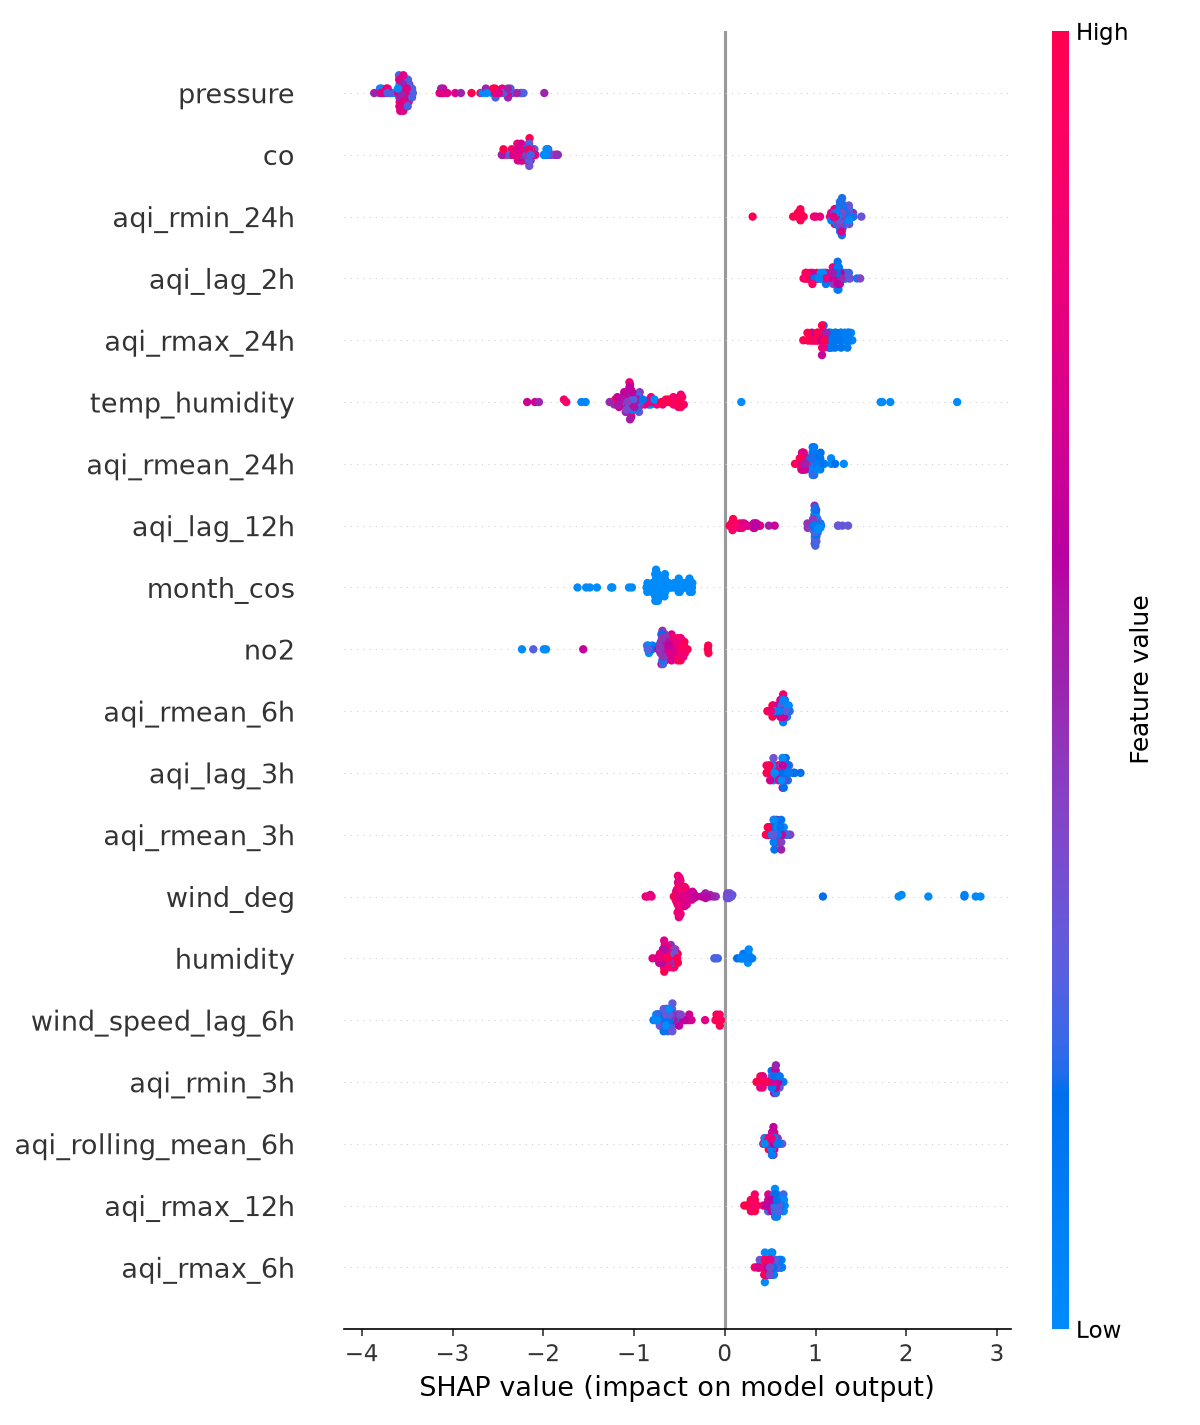
\includegraphics[width=0.86\textwidth]{shap_summary_24h.png}
\caption[SHAP summary, 24-hour horizon]{SHAP summary for the deployed
$+24$\,h Random Forest. Atmospheric \textbf{pressure} is the single strongest
driver (mean $|\text{SHAP}| = 2.96$ AQI points), consistent with pressure
acting as a proxy for the dispersal-versus-inversion regime that determines
whether pollutants accumulate. \textbf{Carbon monoxide} follows at 1.25, a
direct combustion and traffic tracer. The remainder of the top ranks are
dominated by recent AQI history -- the 2-hour lag (1.04), the 24-hour rolling
minimum (0.98) and the 24-hour rolling mean (0.87) -- confirming that at one
day out the model leans heavily on persistence-like information, exactly as the
narrow 7.0\% margin over the persistence baseline would predict.}
\label{fig:shap24}
\end{figure}

\begin{figure}[H]
\centering
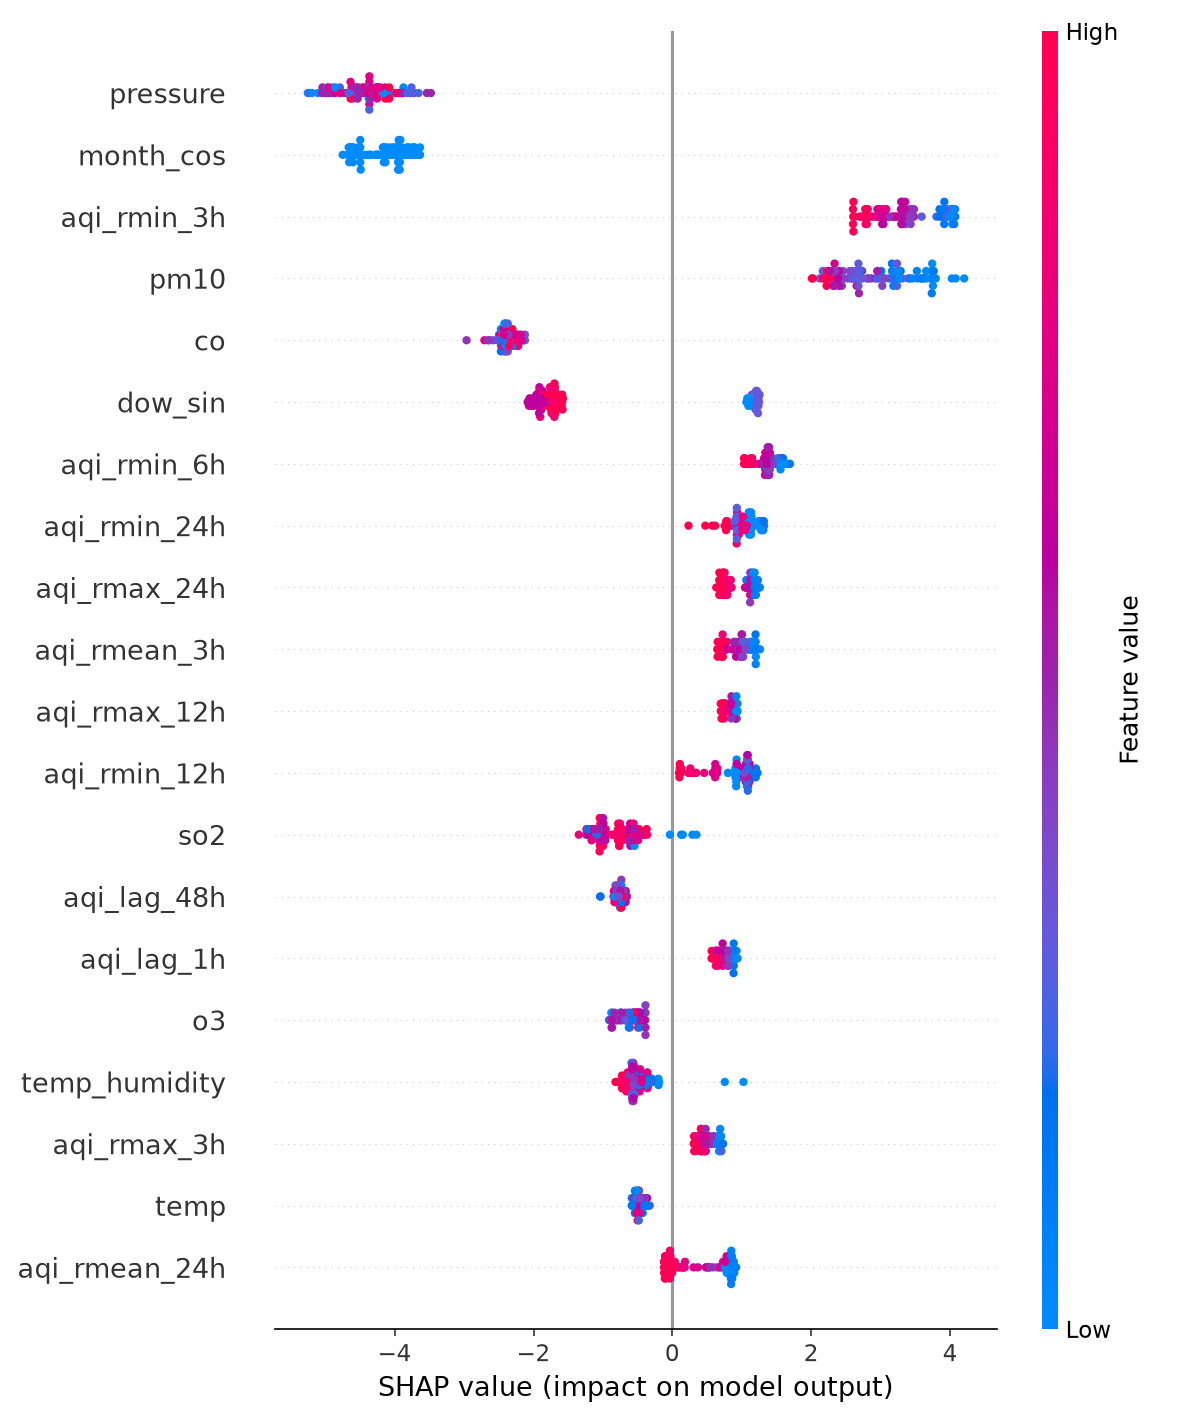
\includegraphics[width=0.86\textwidth]{shap_summary_48h.png}
\caption[SHAP summary, 48-hour horizon]{SHAP summary for the deployed
$+48$\,h Random Forest. The driver set shifts materially. \textbf{Seasonal
phase} (\texttt{month\_cos}, 3.88) becomes the leading feature, \textbf{pressure}
remains strong at 3.53, and \textbf{coarse particulate matter} (\ce{PM10},
3.24) enters the top three alongside \textbf{carbon monoxide} (2.96). Short-window
AQI statistics such as the 3-hour and 6-hour rolling minima are still present
but have been displaced from the top. This is the expected transition: two days
out, the immediate past carries less information than the physical and seasonal
state of the atmosphere.}
\label{fig:shap48}
\end{figure}

\begin{figure}[H]
\centering
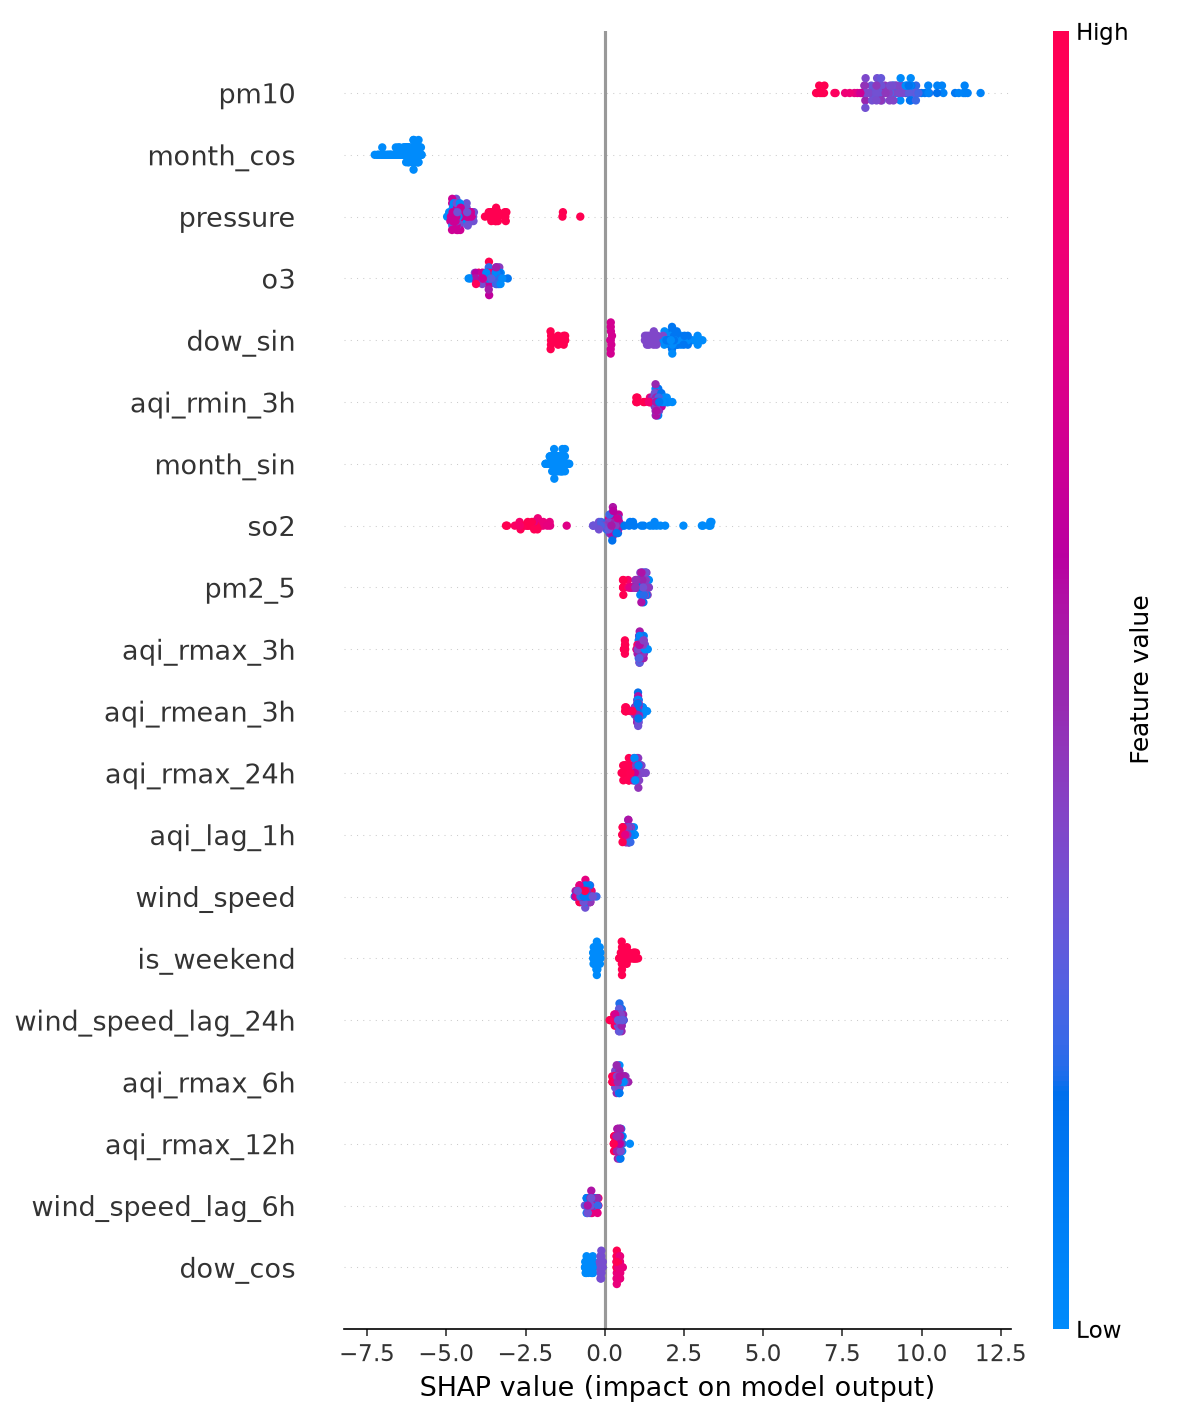
\includegraphics[width=0.86\textwidth]{shap_summary_72h.png}
\caption[SHAP summary, 72-hour horizon]{SHAP summary for the deployed
$+72$\,h Random Forest. The shift away from recent history completes.
\textbf{\ce{PM10}} dominates at 9.05 mean $|\text{SHAP}|$ -- roughly three times
the magnitude of any driver at $+24$\,h -- followed by \textbf{seasonal phase}
(6.60), \textbf{pressure} (4.07) and \textbf{ozone} (3.23). \pmfine appears
at 1.19 and the strongest recent-history term, the 1-hour AQI lag, has fallen to
0.49. At three days out the model is effectively predicting a
climatology-plus-current-loading regime rather than extrapolating a trend,
which is consistent with the low $R^2$ of 0.102 at this horizon.}
\label{fig:shap72}
\end{figure}

\paragraph{Interpretation across horizons.} Read together, the three figures
tell a coherent physical story. As the horizon lengthens, attribution migrates
from \emph{recent AQI dynamics} (lags and short rolling windows at $+24$\,h) to
\emph{atmospheric and seasonal state} (\ce{PM10} loading, pressure, month, ozone
at $+72$\,h). This is exactly the behaviour a well-specified forecasting model
should exhibit: short-range skill comes from momentum, long-range skill comes
from regime.

%=======================================================================
\section{Prediction Mechanism}
%=======================================================================

Both serving surfaces call the same function,
\texttt{predict.get\_forecast()}. The following six steps describe precisely
what happens when a user opens the dashboard or issues
\texttt{GET /forecast}.

\begin{description}[leftmargin=1.4em,style=nextline,itemsep=4pt]

\item[Step 1 -- Load and prepare history.]
\texttt{\_prepared\_history()} reads the entire Parquet feature store,
reindexes it onto a continuous hourly grid via \texttt{to\_hourly\_grid()}, and
applies \texttt{engineer\_features()}. Using the same function as training is
what eliminates train/serve skew. The forecast is then anchored to the most
recent row that carries an \emph{actually measured} AQI, not merely the last
row on the grid -- a grid can legitimately end on placeholder hours that were
never observed. That anchor row's capped AQI becomes
$\text{AQI}(t)$, which is simultaneously the model's reference point and what
the persistence baseline would forecast.

\item[Step 2 -- Compute lag and rolling features.]
Because the anchor is a row of the fully engineered frame, its 64 features
already include every lag, rolling statistic, rate of change and interaction,
computed from the preceding history rather than requested from the model.
Before use, the vector is validated: if any required column is missing, or any
value is null -- the 48-hour lag is undefined until the store holds that much
history -- that horizon is skipped with an explicit, human-readable reason
rather than silently producing a wrong number.

\item[Step 3 -- Scale with the deployed model's own transformer.]
Each registry bundle contains the \texttt{StandardScaler} that was fitted
during that model's final refit, alongside the estimator itself and the exact
ordered list of feature columns. The anchor vector is projected onto that
column order and transformed by that scaler, so the numbers the model sees at
serving time are distributed exactly as they were at training time. For a
sequence model the last \texttt{seq\_len} consecutive hours are stacked into a
single batch instead of a single row.

\item[Step 4 -- Predict the change and reconstruct the level.]
The estimator outputs $\widehat{\Delta}$, the predicted change from the anchor.
\texttt{predict\_with\_interval()} reconstructs the absolute forecast as
$\widehat{\text{AQI}}(t+h) = \text{AQI}(t) + \widehat{\Delta}$ and clips it to
the valid EPA range $[0, 500]$. This runs once per horizon, producing the
$+24$\,h, $+48$\,h and $+72$\,h forecasts.

\item[Step 5 -- Derive an uncertainty band.]
The band is anchored to \texttt{residual\_std}, the standard deviation of the
model's own out-of-sample cross-validation errors -- currently 27.36, 34.75 and
38.79 AQI points for the three horizons. This captures total error, not merely
model variance. For a Random Forest the width is then modulated by how much the
individual trees disagree about \emph{this particular input}: the per-input
spread is divided by the training-set mean spread and clamped to $[0.5, 2.0]$,
so unusual conditions yield visibly wider bands while a single odd input cannot
produce an absurd one. The half-width is $z\sigma$ with $z = 1.2816$, a central
80\% interval. The dashboard labels this as a heuristic band rather than a
calibrated prediction interval, which it is.

\item[Step 6 -- Return a uniform result.]
Each horizon yields the forecast timestamp, point prediction, lower and upper
bounds, EPA category, the serving method, the model name, and the
\texttt{beats\_baseline} verdict. If that verdict is false for a horizon,
\texttt{predict.py} substitutes the persistence forecast with a band derived
from the \emph{baseline's} residual standard deviation, and labels the method
\texttt{"persistence"} so the substitution is visible rather than hidden. The
resulting structure is what FastAPI serialises into its response model and what
Streamlit renders into forecast cards. \textbf{Neither surface contains any
prediction logic of its own}, so the API and the dashboard are guaranteed to
report identical numbers.

\end{description}

%=======================================================================
\section{Automation and CI/CD}
%=======================================================================

\subsection{Workflow Architecture}

Two GitHub Actions workflows constitute the entire operational scheduler.

\begin{table}[H]
\centering
\caption{Scheduled workflows.}
\label{tab:workflows}
\small
\begin{tabular}{@{}p{3.75cm}p{2.15cm}p{8.2cm}@{}}
\toprule
\textbf{Workflow} & \textbf{Schedule} & \textbf{Actions}\\
\midrule
\texttt{feature\_pipeline.yml}
& \texttt{0 * * * *}\newline (hourly)
& Checkout, Python 3.11 with pip cache, install
\texttt{requirements.txt}, run \texttt{src/feature\_pipeline.py} with the
OpenWeather secret and location variables injected, then commit and push
\texttt{data/features.parquet} if it changed.\\
\addlinespace
\texttt{training\_pipeline.yml}
& \texttt{0 3 * * *}\newline (daily, 03:00 UTC)
& Checkout, Python 3.11, install \texttt{requirements.txt} \emph{and}
\texttt{requirements-train.txt} (adding TensorFlow so the LSTM competes), run
\texttt{src/train\_pipeline.py}, then commit and push the refreshed
\texttt{models/} directory. Capped at 90 minutes.\\
\bottomrule
\end{tabular}
\end{table}

Both workflows also expose \texttt{workflow\_dispatch} for manual triggering,
and both are hardened in three ways that matter in practice:

\begin{itemize}[itemsep=2pt]
  \item \textbf{\texttt{permissions: contents: write}}. The default
        \texttt{GITHUB\_TOKEN} is read-only on new repositories, so the
        commit-back step would fail with HTTP 403 without this grant.
  \item \textbf{A shared \texttt{concurrency} group}
        (\texttt{aqi-repo-commit}). Both jobs commit to the same branch and
        would otherwise collide at 03:00 UTC, when their schedules coincide.
        Serialising them eliminates non-fast-forward rejections by
        construction.
  \item \textbf{A rebase-and-retry push loop}. Each job attempts up to three
        pushes, rebasing onto \texttt{origin} with autostash between attempts,
        so a concurrent push cannot lose an hour of data. Commits are tagged
        \texttt{[skip ci]} to prevent a self-triggering loop.
\end{itemize}

Both jobs also guard against the legitimate first-run state in which no
artefacts exist yet -- \texttt{git add} on a missing path is an error, so the
step exits cleanly instead.

\subsection{Evidence of Independent Scheduled Execution}

The automation is not aspirational; it has been running unattended. The
repository's commit history records \textbf{151 commits authored by the
\texttt{aqi-bot} CI identity}, none of them initiated by a human:

\begin{itemize}[itemsep=2pt]
  \item \textbf{146 hourly ``Update features'' commits} from the feature
        pipeline, beginning 2026-09-01 10:33:18 UTC and continuing to
        2026-09-06 02:05:27 UTC.
  \item \textbf{5 daily ``Retrain models'' commits} from the training
        pipeline, at 2026-09-01 10:42:51, 2026-09-02 07:30:37, 2026-09-03
        07:35:20, 2026-09-04 07:35:40 and 2026-09-05 07:18:01 UTC.
\end{itemize}

The hourly cadence is visible directly in consecutive timestamps -- for example
2026-09-05 at 20:01:17, 21:01:18, 22:01:13 and 23:01:18 UTC, then 2026-09-06 at
00:01:26 and 01:01:21 UTC. The retrain commits land on their own daily
schedule, independent of the feature commits, confirming that the two
workflows execute separately. Together these constitute a five-day unbroken
record of a serverless system collecting data and retraining itself with no
manual intervention.

%=======================================================================
\section{Web Application}
%=======================================================================

\subsection{Streamlit Dashboard}

The human interface is a two-page Streamlit application
(\texttt{app/streamlit\_app.py}) with a shared theme
(\texttt{app/theme.py}, palette in \texttt{.streamlit/config.toml}) and a
cached data-access layer (\texttt{app/data\_access.py}) that wraps
\texttt{predict.py} behind \texttt{@st.cache\_data} so a page interaction does
not re-read the store.

\paragraph{Page 1 -- Dashboard (\texttt{app/page\_dashboard.py}).}
The operational view, designed to answer ``what is the air like and what is it
about to do'' without scrolling:
\begin{itemize}[itemsep=1pt]
  \item A \textbf{current AQI gauge}, colour-coded to the EPA category scale,
        with the observation timestamp and a staleness warning if the anchor
        row is more than six hours old.
  \item \textbf{Three forecast cards} for $+24$\,h, $+48$\,h and $+72$\,h,
        each showing the point forecast, its EPA category and colour, and the
        uncertainty band.
  \item A prominent \textbf{alert banner} when the hazard threshold is
        reached (Section~\ref{sec:alerts}).
  \item A \textbf{key pollutant grid} giving current concentrations for
        \pmfine, \ce{PM10}, \ce{O3}, \ce{NO2}, \ce{SO2} and \ce{CO}, plus
        the identified dominant pollutant.
  \item A \textbf{recent-trend sparkline} and the \textbf{top SHAP drivers}
        for the active forecast.
\end{itemize}

\paragraph{Page 2 -- Model Analysis (\texttt{app/page\_analysis.py}).}
The transparency view, for a user who wants to know whether to believe the
forecast:
\begin{itemize}[itemsep=1pt]
  \item A \textbf{14-day historical AQI chart} with forecast points and
        uncertainty bands overlaid.
  \item A \textbf{model accuracy comparison} rendered live from the registry's
        \texttt{metrics\_*.json} -- RMSE, MAE and $R^2$ per horizon against
        the persistence baseline, so the numbers in
        Table~\ref{tab:results} are visible in the product itself.
  \item A \textbf{SHAP explainability panel} showing the summary plot and
        ranked feature importances per horizon, with the staleness flag from
        \texttt{predict.shap\_plot\_status()} surfaced to the user.
\end{itemize}

\subsection{FastAPI Backend}

\texttt{api/main.py} exposes the same capabilities as a machine interface,
with Pydantic response models and auto-generated OpenAPI documentation at
\texttt{/docs}.

\begin{table}[H]
\centering
\caption{REST API endpoints.}
\label{tab:api}
\small
\begin{tabular}{@{}p{4.1cm}p{10.2cm}@{}}
\toprule
\textbf{Endpoint} & \textbf{Purpose}\\
\midrule
\texttt{GET /health} & Liveness probe: feature store row count and which
horizons currently have loadable models.\\
\texttt{GET /current} & Latest measured AQI, EPA category, dominant
pollutant, observation age and staleness flag.\\
\texttt{GET /forecast} & Three-day forecast with uncertainty bands, serving
method and baseline verdict per horizon.\\
\texttt{GET /history?hours=} & Recent observed AQI series (default 336 hours,
i.e.\ 14 days).\\
\texttt{GET /alerts} & Whether hazardous air is currently measured or
forecast, with the triggering horizon and a human-readable message.\\
\texttt{GET /metrics} & Per-horizon model metrics and baseline comparison,
read from the registry.\\
\texttt{GET /categories} & The full EPA category table with alerting flags.\\
\texttt{GET /categories/\{aqi\}} & Classify an arbitrary AQI value.\\
\bottomrule
\end{tabular}
\end{table}

Because both surfaces delegate to \texttt{predict.py}, the dashboard and the
API are structurally incapable of reporting different forecasts.

\subsection{Deployed Interface}

Figures~\ref{fig:dash} and~\ref{fig:analysis} show the live application,
captured on 6 September 2026 against the feature store and model registry
described throughout this report. Each page is presented as a two-panel scroll
capture, since both are taller than a single browser viewport.

\begin{figure}[H]
\centering
\begin{subfigure}[t]{\linewidth}
  \centering
  \makebox[\linewidth][c]{\fbox{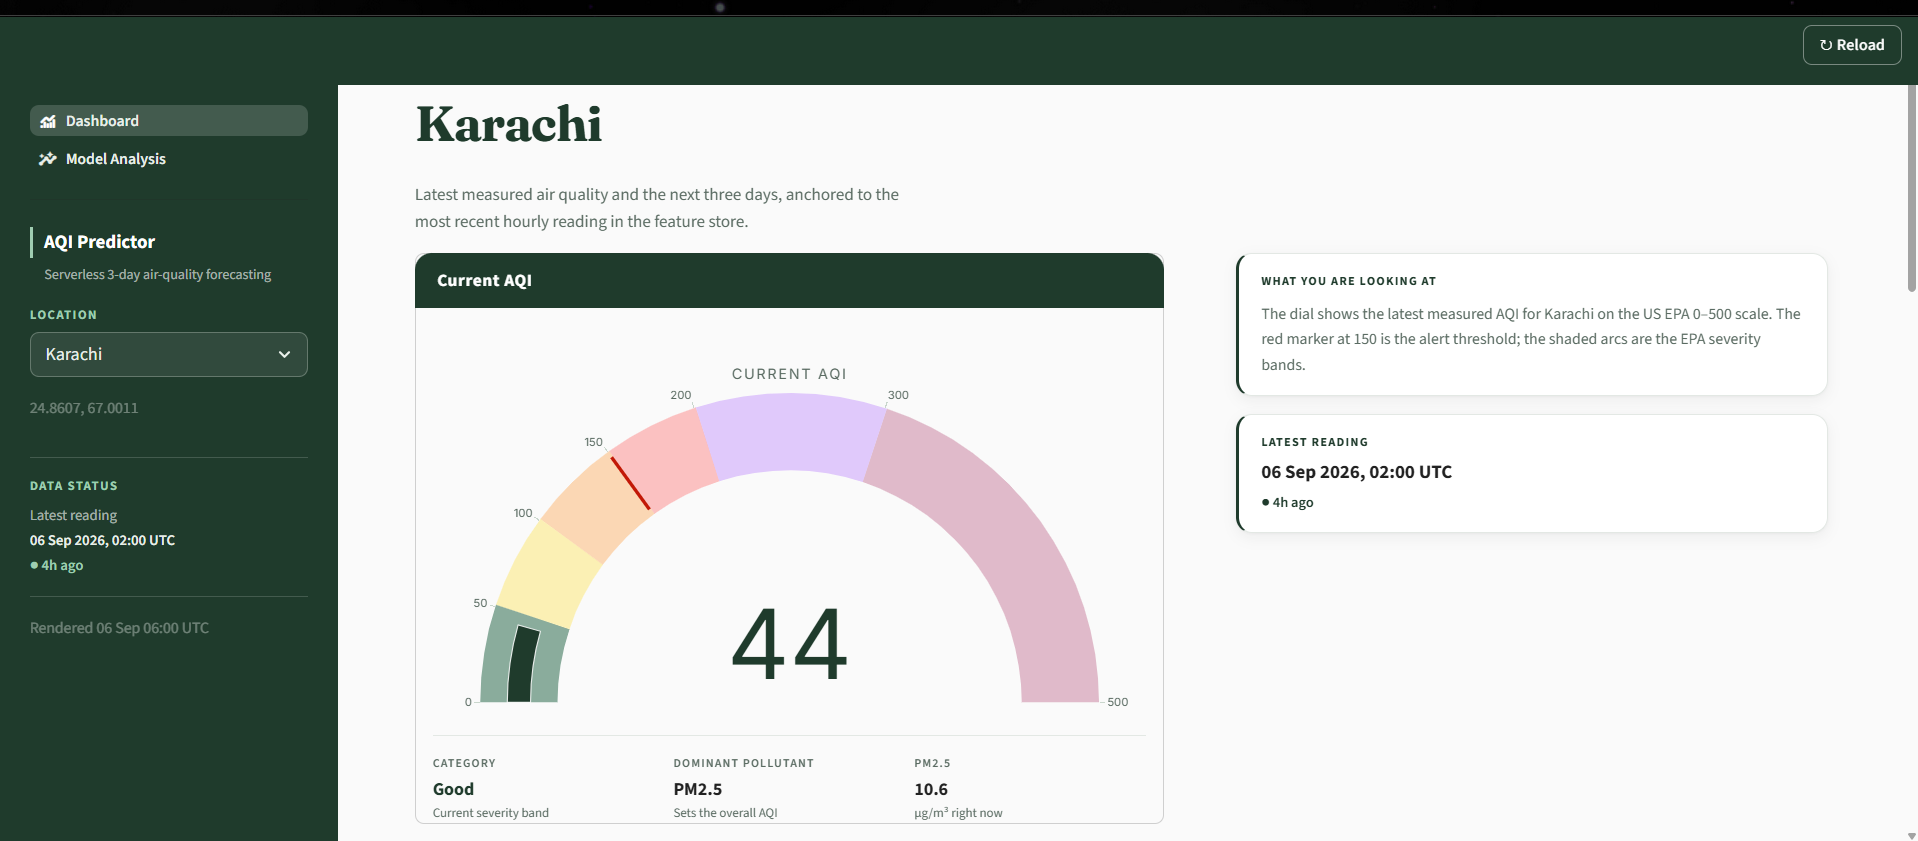
\includegraphics[width=1.12\linewidth]{dashboard_full1.png}}}
  \caption{Upper panel: current-conditions hero and AQI gauge.}
  \label{fig:dash-a}
\end{subfigure}

\vspace{0.45cm}
\begin{subfigure}[t]{\linewidth}
  \centering
  \makebox[\linewidth][c]{\fbox{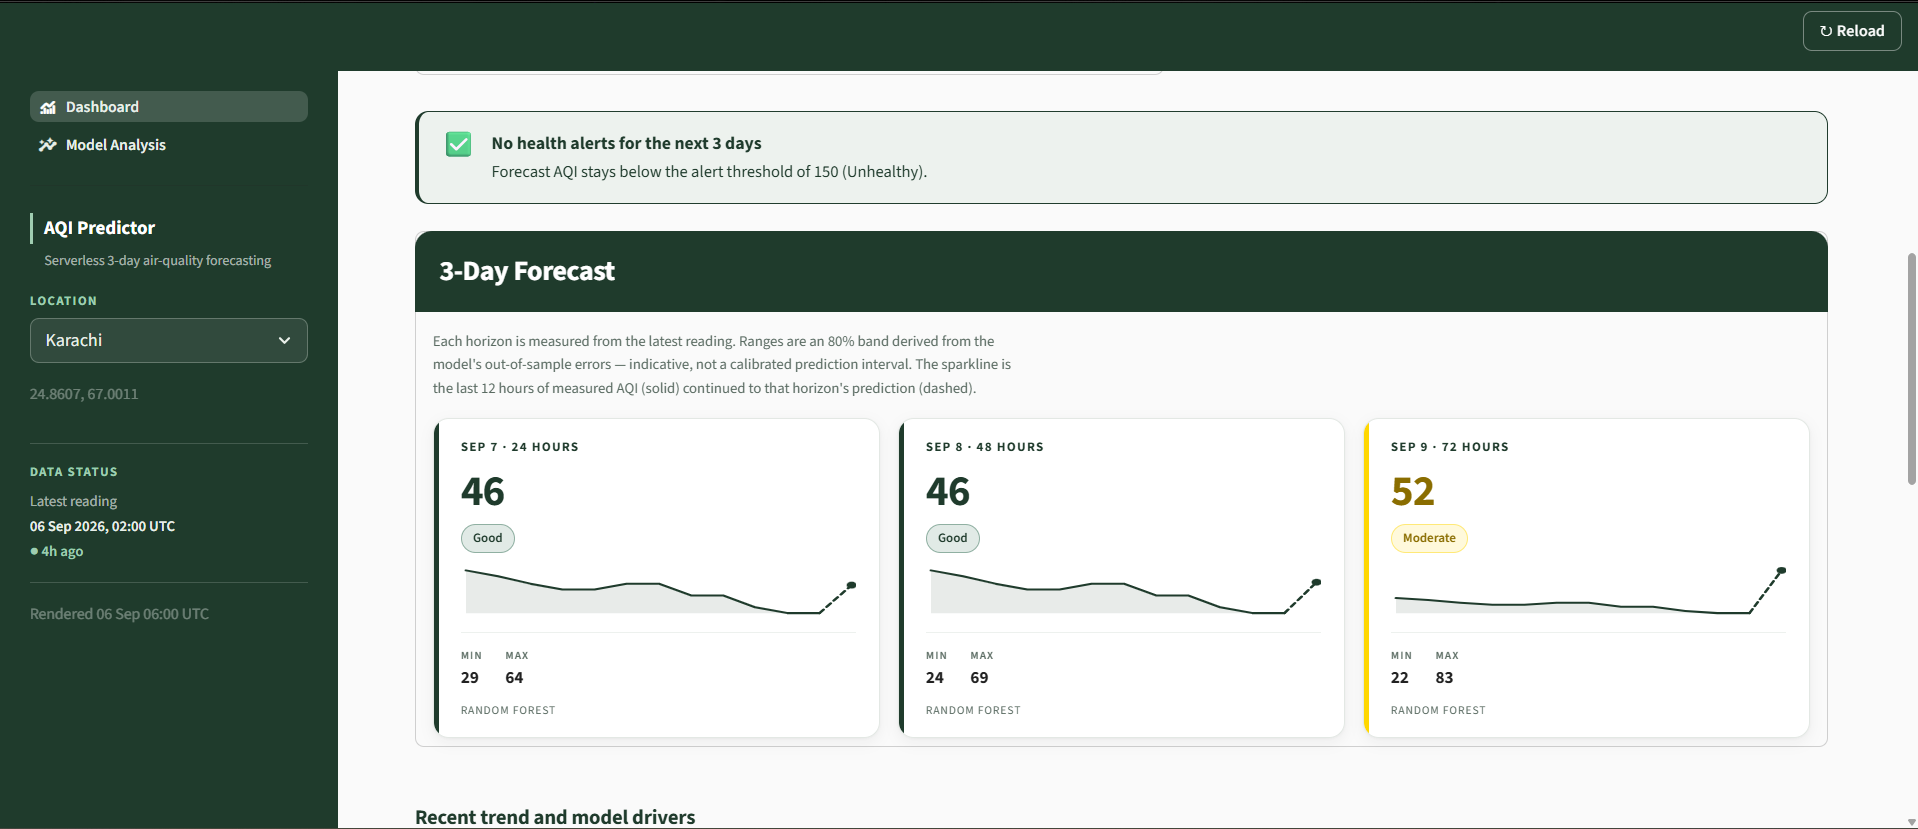
\includegraphics[width=1.12\linewidth]{dashboard_full2.png}}}
  \caption{Lower panel: alert state and three-day forecast cards.}
  \label{fig:dash-b}
\end{subfigure}
\caption[Dashboard page]{\textbf{Dashboard page, full view} of the deployed
Streamlit application. \textbf{(a)} The gauge renders the latest measured AQI
of 44 on the EPA 0--500 scale, with the shaded arcs marking the severity bands
and the red marker fixed at the alert threshold of 150. Beneath it the page
reports the category (\emph{Good}), the dominant pollutant driving the index
(\pmfine) and its concentration
(\SI{10.6}{\micro\gram\per\cubic\metre}). The sidebar carries the location
selector, the coordinates, and a data-status block showing the reading is four
hours old. \textbf{(b)} The alert region is in its non-triggered state --
``No health alerts for the next 3 days'' -- because the forecast stays below
150. The three forecast cards give 46 (\emph{Good}) at $+24$\,h, 46
(\emph{Good}) at $+48$\,h and 52 (\emph{Moderate}) at $+72$\,h, each with its
80\% band (29--64, 24--69 and 22--83 respectively) and each labelled
\textsc{random forest}, matching the deployment decision recorded in
Table~\ref{tab:baseline}. Note how the bands widen with horizon, a direct
visual consequence of the growing residual standard deviations reported in
Section~\ref{sec:delta}.}
\label{fig:dash}
\end{figure}

\begin{figure}[H]
\centering
\begin{subfigure}[t]{\linewidth}
  \centering
  \makebox[\linewidth][c]{\fbox{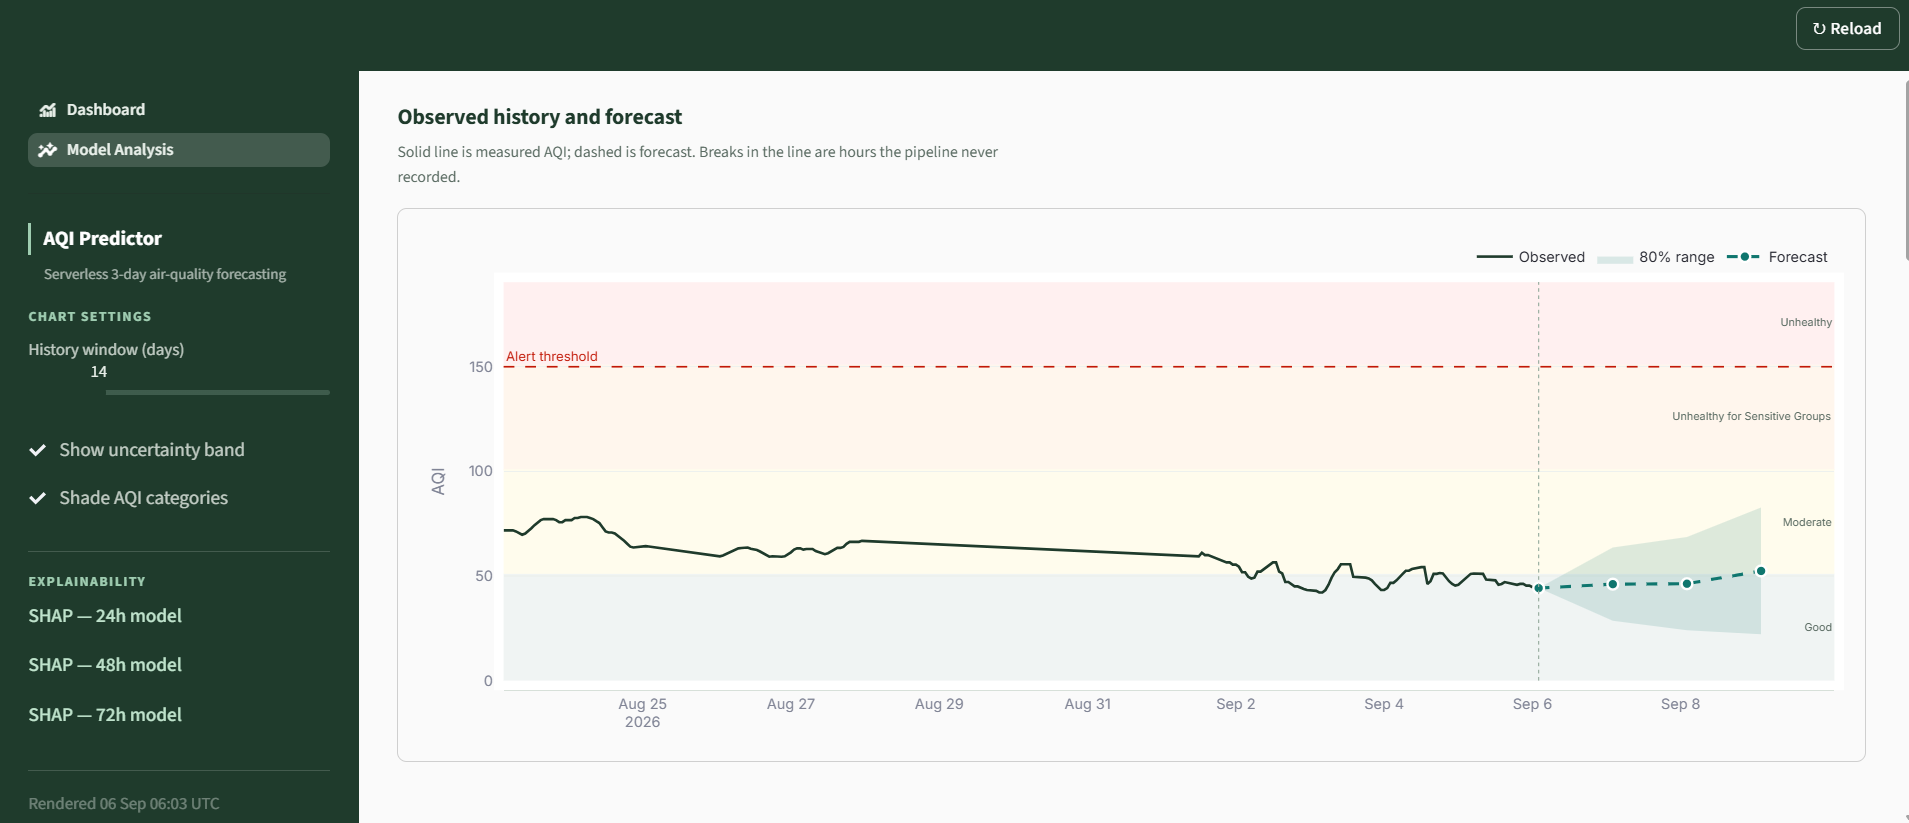
\includegraphics[width=1.12\linewidth]{analysis_full1.png}}}
  \caption{Upper panel: observed history with forecast and uncertainty band.}
  \label{fig:analysis-a}
\end{subfigure}

\vspace{0.45cm}
\begin{subfigure}[t]{\linewidth}
  \centering
  \makebox[\linewidth][c]{\fbox{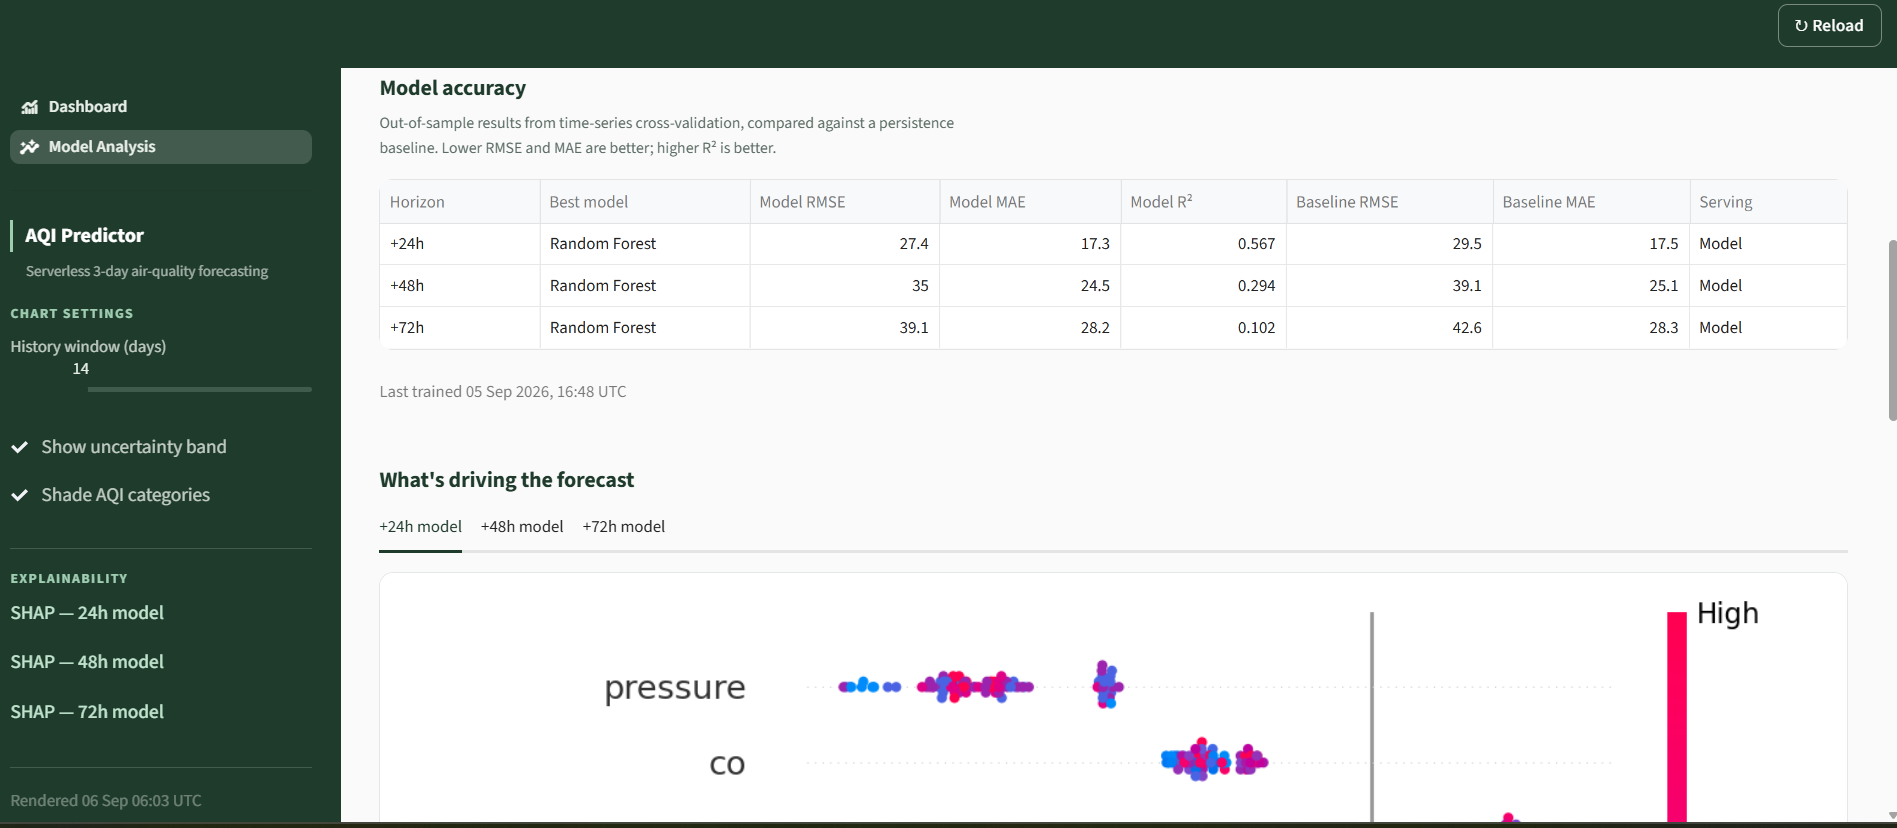
\includegraphics[width=1.12\linewidth]{analysis_full2.png}}}
  \caption{Lower panel: model accuracy table and SHAP explainability panel.}
  \label{fig:analysis-b}
\end{subfigure}
\caption[Model Analysis page]{\textbf{Model Analysis page, full view} of the
deployed application. \textbf{(a)} Fourteen days of measured AQI (solid line)
continue into the three-day forecast (dashed) with its shaded 80\% range. The
background is shaded by EPA category and the red dashed rule marks the alert
threshold at 150, placing the current regime visually well inside the
\emph{Good} and \emph{Moderate} bands. The sidebar exposes the history window,
uncertainty-band and category-shading toggles, and per-horizon SHAP links.
\textbf{(b)} The accuracy table is rendered live from
\texttt{models/metrics\_*.json} and reproduces exactly the figures in
Table~\ref{tab:results} -- RMSE 27.4, MAE 17.3 and $R^2$ 0.567 at $+24$\,h
against a baseline RMSE of 29.5, and so on for the longer horizons -- with a
\texttt{Serving} column confirming all three horizons serve the trained model
rather than the baseline. The footer records the registry's training time of
05 Sep 2026, 16:48 UTC. Below, the ``What's driving the forecast'' panel shows
the SHAP beeswarm for the selected horizon, with \texttt{pressure} and
\texttt{co} as the leading $+24$\,h drivers, agreeing with
Figure~\ref{fig:shap24}.}
\label{fig:analysis}
\end{figure}

\begin{figure}[H]
\centering
\makebox[\linewidth][c]{\fbox{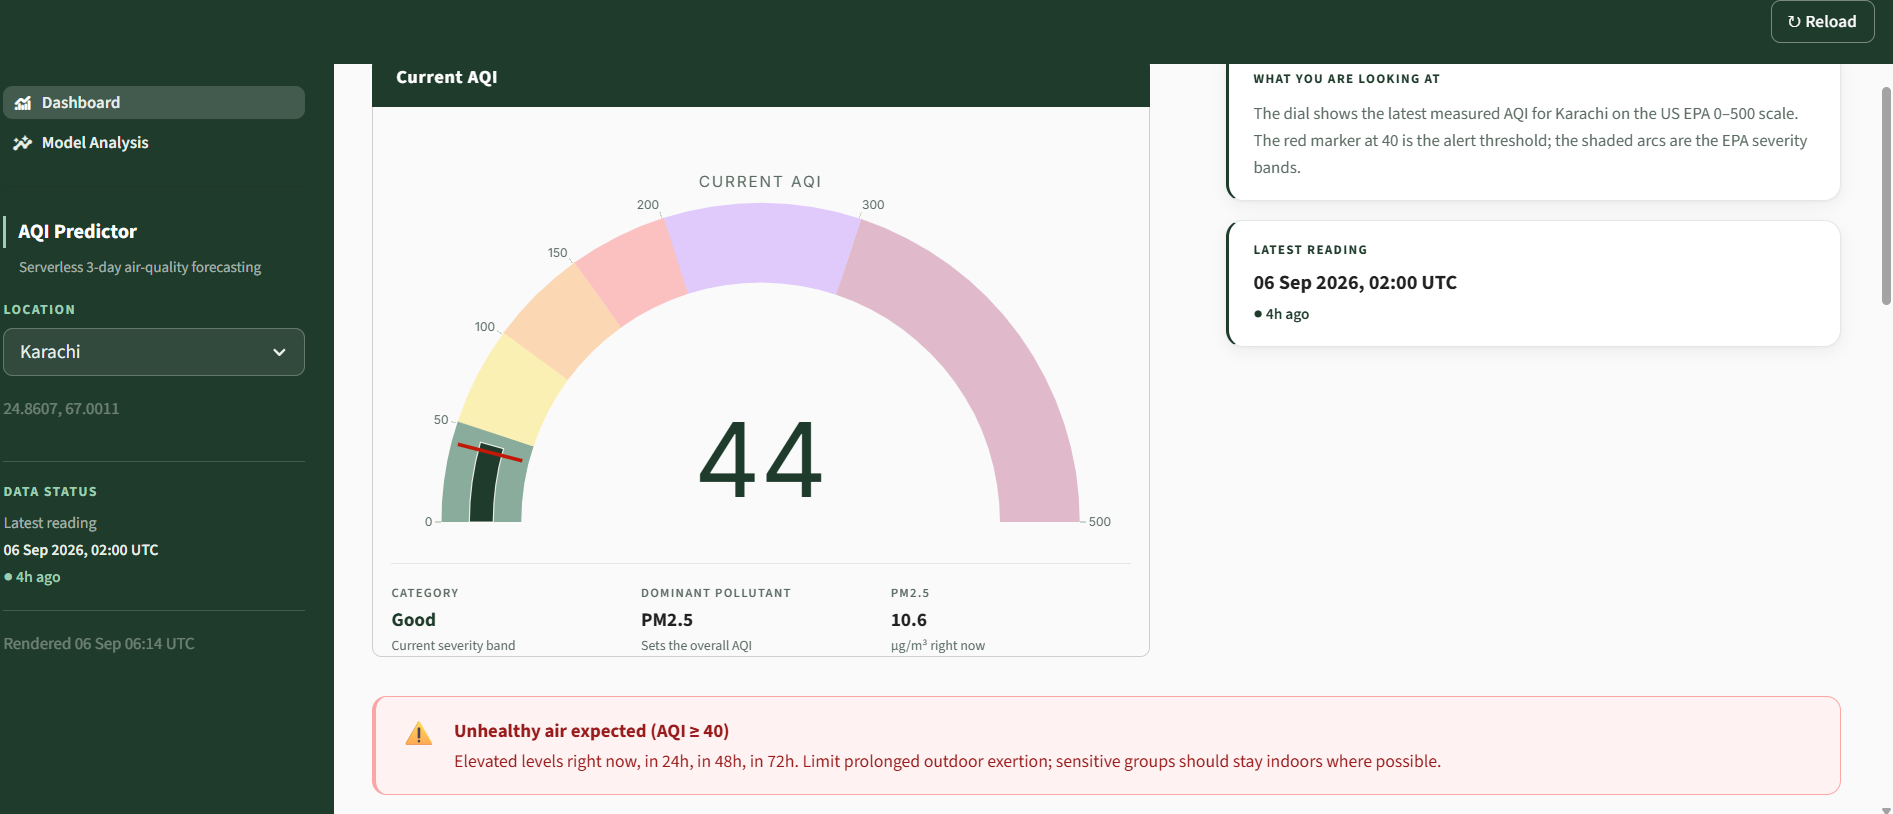
\includegraphics[width=1.12\linewidth]{alert_banner.png}}}
\caption[Alert banner, triggered state]{\textbf{Dashboard page,
alert-triggered state}, showing the red hazard banner and the gauge's
threshold marker. The banner names every offending horizon --
``Elevated levels right now, in 24h, in 48h, in 72h'' -- and pairs it with
the public-health advice to limit prolonged outdoor exertion. Karachi's air
remained in the \emph{Good} to \emph{Moderate} range throughout the capture
window (measured AQI 44.2; forecasts 46.1, 46.3 and 52.4), so no genuine
exceedance of the production threshold was available to photograph. The
threshold was therefore lowered temporarily purely to exercise the alerting
path, which is why the banner text and the gauge marker read a reduced value
rather than 150. The alerting \emph{logic} shown is exactly the deployed
logic; only the constant differs, and the production value of
\texttt{ALERT\_THRESHOLD = 150} was restored immediately afterwards --
Figure~\ref{fig:dash-a} shows the same gauge with the marker back at 150.}
\label{fig:alert}
\end{figure}

%=======================================================================
\section{Alerts System}
\label{sec:alerts}
%=======================================================================

\subsection{Threshold Logic}

Alerting is grounded in the published US EPA category scale rather than an
arbitrary cutoff. \texttt{config.py} encodes the six official bands as
half-open intervals, $\text{lo} \le \text{AQI} < \text{hi}$, so that a
fractional value such as 50.4 cannot fall between two categories; the final
band is closed at the top and absorbs anything above 500
(Table~\ref{tab:epa}).

\begin{table}[H]
\centering
\caption{EPA AQI categories as implemented, with alerting status.}
\label{tab:epa}
\small
\begin{tabular}{@{}llc@{}}
\toprule
\textbf{AQI range} & \textbf{Category} & \textbf{Triggers alert}\\
\midrule
$0 \le \text{AQI} < 51$    & Good & \\
$51 \le \text{AQI} < 101$  & Moderate & \\
$101 \le \text{AQI} < 151$ & Unhealthy for Sensitive Groups & \\
$151 \le \text{AQI} < 201$ & Unhealthy & \checkmark\\
$201 \le \text{AQI} < 301$ & Very Unhealthy & \checkmark\\
$301 \le \text{AQI} \le 501$ & Hazardous & \checkmark\\
\bottomrule
\end{tabular}
\end{table}

The alert threshold is set at \texttt{ALERT\_THRESHOLD = 150}, the entry point
of the EPA's \emph{Unhealthy} classification. This is the correct trigger point
for a public-health warning: below it, EPA guidance concerns sensitive groups
only, whereas at and above it the agency advises that members of the
\emph{general} population may begin to experience adverse effects. Anchoring
the threshold to a published standard rather than a hand-tuned number means the
alert carries an externally-defined meaning.

\subsection{Surfacing the Alert}

An alert fires if \emph{either} the latest measured AQI \emph{or} any of the
three forecast values reaches the threshold. Alerting on the forecast, not only
on the observation, is the entire point of the system -- a warning that arrives
after the episode has begun has no preventive value.

The condition is evaluated in two places against the same threshold constant:

\begin{itemize}[itemsep=2pt]
  \item \textbf{In the dashboard}, as a prominent full-width banner directly
        beneath the gauge on the Dashboard page. The banner is always rendered
        in one of four fixed severity treatments, so the state is legible
        before any text is read: a red \texttt{danger} style when the
        threshold is reached (Figure~\ref{fig:alert}) and a green
        \texttt{ok} style confirming ``No health alerts for the next 3 days''
        when it is not (Figure~\ref{fig:dash-b}). The message names every
        offending horizon and adds the corresponding public-health advice.
  \item \textbf{Through the API}, at \texttt{GET /alerts}, which returns a
        boolean trigger flag, the threshold in force, the horizon responsible,
        and a human-readable message -- either ``Unhealthy air (AQI $\ge$ 150)
        expected \ldots'' naming the offending horizon, or a confirmation that
        no reading at or above the threshold is measured or forecast. The same
        flag is echoed in the \texttt{/forecast} response, and
        \texttt{/categories} annotates every band with whether it alerts, so a
        downstream consumer can reproduce the logic exactly.
\end{itemize}

%=======================================================================
\section{Deployment}
%=======================================================================

The dashboard runs live on \textbf{Streamlit Community Cloud}, bound directly
to the GitHub repository. There is no build server, container registry or
deployment script: Streamlit Cloud watches the \texttt{main} branch, and any
push -- whether a human code change or an \texttt{aqi-bot} commit from the
hourly feature pipeline -- triggers a rebuild and redeploy. Continuous
deployment is therefore a property of the hosting arrangement rather than
something the project implements.

This closes the serverless loop. GitHub Actions collects data and retrains
models, committing both back to the repository; Streamlit Cloud redeploys from
that same repository; and the deployed app reads the feature store and model
registry straight out of its own checkout. No component of the running system
requires a machine that anyone administers.

\paragraph{Keeping the serving environment lightweight.}
Dependencies are split deliberately across two files so that training weight
never reaches production:

\begin{itemize}[itemsep=2pt]
  \item \texttt{requirements.txt} is the \textbf{serving stack} -- pandas,
        NumPy, scikit-learn, joblib, \texttt{pyarrow}, Streamlit, Plotly,
        FastAPI, Uvicorn, Matplotlib, SHAP and the Hopsworks client. This is
        the only file Streamlit Cloud installs.
  \item \texttt{requirements-train.txt} adds \texttt{tensorflow-cpu}, and is
        installed \emph{only} by the daily training workflow and by developers
        who intend to retrain.
\end{itemize}

The split is safe precisely because the deployed models are Random Forest
joblibs at every horizon: \texttt{predict.py} imports TensorFlow lazily and
only when a bundle is flagged as a sequence model, so the serving path never
touches it. Excluding a multi-hundred-megabyte dependency keeps Streamlit
Cloud builds inside their resource limits and materially reduces cold-start
time.

\paragraph{Reproducibility measures.}
\texttt{runtime.txt} pins Streamlit Cloud to Python 3.11, matching the CI
runners. scikit-learn is pinned to an exact version (1.9.0) rather than a
range, because a joblib artefact records the scikit-learn version that produced
it: allowing CI and local environments to drift across minor versions produced
\texttt{InconsistentVersionWarning} on load. Other libraries carry lower bounds
for reproducibility and upper bounds on the majors known to break this code,
and \texttt{hopsworks[python]} is pinned to the connected backend's minor
series (5.0.x). Finally, Keras artefact paths are always reconstructed locally
by \texttt{config.keras\_model\_path()} rather than read from the bundle, so a
CI absolute path such as \texttt{/home/runner/work/\ldots} can never break a
load on another machine.

%=======================================================================
\section{Results Summary}
%=======================================================================

Table~\ref{tab:requirements} maps each original project requirement to its
implementation and to the concrete evidence of fulfilment.

\begin{longtable}{@{}p{2.9cm}p{3.6cm}p{7.6cm}@{}}
\caption{Requirement fulfilment matrix.}
\label{tab:requirements}\\
\toprule
\textbf{Requirement} & \textbf{Implementation} & \textbf{Evidence of fulfilment}\\
\midrule
\endfirsthead
\multicolumn{3}{@{}l}{\small\itshape (Table \ref{tab:requirements} continued)}\\
\toprule
\textbf{Requirement} & \textbf{Implementation} & \textbf{Evidence of fulfilment}\\
\midrule
\endhead
\bottomrule
\endlastfoot

Feature pipeline
& \texttt{src/feature\_pipeline.py}
& Runs hourly on GitHub Actions; fetches OpenWeather pollution and weather,
computes EPA AQI from per-pollutant sub-indices, merges idempotently into the
store. 146 automated feature commits recorded.\\
\addlinespace

Historical backfill
& \texttt{src/backfill.py}
& \num{8835} hourly rows spanning 368 days (2025-09-03 to 2026-09-06), 100\%
measured with no imputation and no gap exceeding one hour. Full lineage in
\texttt{data/PROVENANCE.md} with SHA-256 checksums and retained raw API
responses.\\
\addlinespace

Feature store
& \texttt{data/features.parquet} + Hopsworks \texttt{aqi\_features} v2
& Dual-write design: Parquet as dependency-free source of truth, managed
Hopsworks feature group via Kafka stream ingestion with \texttt{timestamp} as
primary key and event time. Fail-soft coupling verified by unit tests.\\
\addlinespace

Training pipeline with RMSE / MAE / $R^2$
& \texttt{src/train\_pipeline.py}
& Four candidate families $\times$ three horizons under five-fold
expanding-window \texttt{TimeSeriesSplit} with horizon-length gap. All twelve
candidate results plus per-fold breakdowns recorded in
\texttt{models/metrics\_*.json} (Table~\ref{tab:results}).\\
\addlinespace

Model registry and automatic selection
& \texttt{models/}
& Best model per horizon selected by pooled out-of-sample RMSE, refit on all
data, serialised with its scaler, feature list and residual statistics. Random
Forest deployed at all three horizons.\\
\addlinespace

Baseline comparison
& \texttt{beats\_baseline} in registry
& Persistence baseline scored on identical folds. RMSE reduced by 7.0\%
($+24$\,h), 10.5\% ($+48$\,h) and 8.1\% ($+72$\,h); all three verdicts
\texttt{true}, so all three serve their trained model
(Table~\ref{tab:baseline}).\\
\addlinespace

CI/CD automation
& \texttt{.github/workflows/}
& Hourly feature workflow and daily 03:00 UTC training workflow, both
serverless, with shared concurrency locking and rebase-retry pushes. 151
autonomous \texttt{aqi-bot} commits over five days.\\
\addlinespace

Interactive dashboard with forecast and alerts
& \texttt{app/}
& Two-page Streamlit app: gauge, three forecast cards with uncertainty bands,
pollutant grid, trend sparkline, and historical/accuracy/SHAP analysis page.
Live on Streamlit Community Cloud with continuous deployment.\\
\addlinespace

REST API
& \texttt{api/main.py}
& Eight FastAPI endpoints with Pydantic models and OpenAPI docs, sharing
\texttt{predict.py} with the dashboard so the two cannot diverge.\\
\addlinespace

Exploratory data analysis
& \texttt{notebooks/eda.py}
& Three regenerable figures in \texttt{data/eda/} establishing diurnal
seasonality, particulate dominance and autocorrelation structure
(Figure~\ref{fig:eda}).\\
\addlinespace

Explainability
& SHAP \texttt{TreeExplainer}
& Per-horizon summary plots and ranked importance JSON regenerated each
training run, displayed in the dashboard with automatic staleness detection
(Figures~\ref{fig:shap24}--\ref{fig:shap72}).\\
\addlinespace

Alerts
& \texttt{ALERT\_THRESHOLD = 150}
& EPA \emph{Unhealthy} threshold applied to both measured and forecast AQI;
surfaced as a colour-coded dashboard banner and via \texttt{GET /alerts}.\\
\addlinespace

Uncertainty quantification
& \texttt{predict\_with\_interval()}
& Central 80\% bands ($z = 1.2816$) from out-of-sample residual standard
deviations of 27.36, 34.75 and 38.79 AQI points, modulated per input by
Random Forest tree disagreement.\\
\end{longtable}

%=======================================================================
\section{Limitations and Future Work}
%=======================================================================

\paragraph{Single-location scope.}
The system currently forecasts for Karachi alone. This is a configuration
choice, not an architectural constraint: location is read from environment
variables (\texttt{AQI\_CITY}, \texttt{AQI\_LAT}, \texttt{AQI\_LON}) and
\texttt{config.py} already carries presets for Lahore, Islamabad, Peshawar,
Quetta and Delhi. Extending to multiple cities means partitioning the feature
store by location and training per-location models; the ingestion, training,
serving and automation layers need no redesign. A shared multi-city model with
location as a feature is the more interesting version, since it would let
sparse-history cities borrow strength from dense ones.

\paragraph{Forecast weather as an input.}
This is the single highest-leverage enhancement available. The models currently
condition on \emph{current-time} features -- present pollutant loading, present
weather, and the recent history of both -- and must implicitly infer the
atmospheric evolution of the next one to three days. Yet that evolution is
partly knowable: both OpenWeather and Open-Meteo expose free forecast
endpoints. Supplying \emph{forecast} temperature, wind, humidity and pressure
at the target hour as explicit inputs would replace inference with information,
and the SHAP analysis suggests exactly where the gain would land: at $+72$\,h
the model already leans on pressure and seasonal phase as proxies for regime,
which is precisely the signal a weather forecast would provide directly. The
training pipeline would need no structural change -- only additional feature
columns and a matching change to the serving feature assembly.

\paragraph{Accumulating historical volume.}
368 days of history is sufficient to learn a diurnal cycle and one pass through
the seasons, but not to distinguish a genuine seasonal pattern from a
single-year anomaly. The consequence is visible in the per-fold metrics, where
the earliest expanding-window fold trains on one season and is scored on
another. This limitation resolves itself: the hourly pipeline adds 24 rows per
day unattended, so multi-year coverage accrues without further effort, and each
nightly retrain automatically benefits. Once the store spans several years, two
things become worth revisiting -- predicting the absolute AQI level rather than
the delta, and giving sequence models such as the LSTM or a Temporal Fusion
Transformer enough data to compete on their own terms.

\paragraph{Averaging windows in the AQI conversion.}
The EPA defines its breakpoints against averaging windows the data source does
not provide -- 24 hours for particulates, 8 hours for ozone and carbon
monoxide. Instantaneous hourly readings are used as a proxy, which biases the
computed AQI high during short spikes. Because concentrations are stored raw
and \texttt{src/repair\_feature\_store.py} can recompute the AQI column in
place, implementing proper trailing-window averages is a contained change that
would improve fidelity to the standard.

\paragraph{Calibrated prediction intervals.}
The current bands are an honest heuristic combining out-of-sample residual
spread with ensemble disagreement, and are labelled as such. Quantile
regression forests or conformal prediction would provide intervals with
guaranteed empirical coverage, which matters if the forecast is ever used for
formal decision-making rather than public information.

%=======================================================================
\section{Conclusion}
%=======================================================================

The Pearls AQI Predictor demonstrates that a complete, continuously-operating
machine learning system -- ingestion, feature store, automated retraining,
model registry, explainability, REST API and interactive dashboard -- can be
built and run with no managed infrastructure whatsoever. Every scheduled
component executes on GitHub Actions, every artefact is versioned in Git, and
the user interface redeploys itself from the same repository. The
infrastructure cost is zero and there is no server for anyone to administer.

The system's substance rests on genuine data and honest evaluation. The feature
store holds \num{8835} consecutive hourly observations covering 368 days,
entirely measured, with lineage documented down to SHA-256 checksums and
retained raw API responses. Four model families were placed in competition at
each of three horizons under expanding-window time-series cross-validation with
a horizon-length gap to prevent leakage, and every candidate's metrics were
recorded rather than only the winner's. Random Forest was selected at all three
horizons on out-of-sample RMSE, beating a persistence baseline by 7.0\%,
10.5\% and 8.1\% at $+24$\,h, $+48$\,h and $+72$\,h. Crucially, the
architecture would have refused to deploy a model that did \emph{not} beat
persistence, falling back to the baseline and saying so.

Beyond the metrics, the design choices that most define the system are the ones
that protect correctness: a single shared feature-engineering function used by
both training and serving, eliminating skew by construction; a single
prediction module behind both the API and the dashboard, making disagreement
between them impossible; and SHAP artefacts that are timestamp-checked against
the models they claim to explain. The resulting SHAP analysis shows attribution
migrating from recent AQI momentum at $+24$\,h to particulate loading and
seasonal regime at $+72$\,h -- the physically coherent behaviour a
well-specified forecasting model should exhibit, and evidence that the models
have learned mechanism rather than coincidence.

Three days of air quality forecasting for a city of twenty million people, on
zero infrastructure, retraining itself nightly. The remaining path to improved
accuracy is clear and largely mechanical: feed the models forecast weather
instead of asking them to infer it, and let the hourly pipeline keep
accumulating history.

%=======================================================================
\section*{References}
\addcontentsline{toc}{section}{References}
%=======================================================================

\begin{thebibliography}{99}
\small

\bibitem{openweather}
OpenWeather. \emph{Air Pollution API}.
\url{https://openweathermap.org/api/air-pollution}

\bibitem{openweather-hist}
OpenWeather. \emph{Air Pollution API -- Historical Data}.
\url{https://openweathermap.org/api/air-pollution#history}

\bibitem{openmeteo}
Open-Meteo. \emph{Historical Weather API (ERA5 Archive)}.
\url{https://open-meteo.com/en/docs/historical-weather-api}

\bibitem{epa}
United States Environmental Protection Agency.
\emph{Technical Assistance Document for the Reporting of Daily Air Quality --
the Air Quality Index (AQI)}. EPA-454/B-24-002.
\url{https://www.airnow.gov/aqi/aqi-basics/}

\bibitem{hopsworks}
Hopsworks. \emph{Hopsworks Feature Store Documentation}.
\url{https://docs.hopsworks.ai/}

\bibitem{hopsworks-stream}
Hopsworks. \emph{Feature Group Stream Ingestion (\texttt{stream=True})}.
\url{https://docs.hopsworks.ai/latest/user_guides/fs/feature_group/create/}

\bibitem{sklearn}
Pedregosa, F. et al. (2011). Scikit-learn: Machine Learning in Python.
\emph{Journal of Machine Learning Research}, 12, 2825--2830.
\url{https://scikit-learn.org/stable/}

\bibitem{sklearn-tscv}
Scikit-learn Developers. \emph{TimeSeriesSplit -- Cross-validation for Time
Series Data}.
\url{https://scikit-learn.org/stable/modules/generated/sklearn.model_selection.TimeSeriesSplit.html}

\bibitem{tensorflow}
Abadi, M. et al. (2016). TensorFlow: A System for Large-Scale Machine
Learning. \emph{12th USENIX Symposium on Operating Systems Design and
Implementation (OSDI '16)}, 265--283.
\url{https://www.tensorflow.org/}

\bibitem{keras}
Chollet, F. et al. (2015). \emph{Keras}.
\url{https://keras.io/api/layers/recurrent_layers/lstm/}

\bibitem{lundberg}
Lundberg, S. M. and Lee, S.-I. (2017). A Unified Approach to Interpreting Model
Predictions. \emph{Advances in Neural Information Processing Systems 30
(NeurIPS 2017)}, 4765--4774.

\bibitem{shap-tree}
Lundberg, S. M., Erion, G. G. and Lee, S.-I. (2020). From Local Explanations to
Global Understanding with Explainable AI for Trees.
\emph{Nature Machine Intelligence}, 2(1), 56--67.
\url{https://shap.readthedocs.io/}

\bibitem{breiman}
Breiman, L. (2001). Random Forests. \emph{Machine Learning}, 45(1), 5--32.

\bibitem{streamlit}
Streamlit Inc. \emph{Streamlit Documentation} and
\emph{Streamlit Community Cloud}.
\url{https://docs.streamlit.io/}

\bibitem{fastapi}
Ram\'irez, S. \emph{FastAPI Documentation}.
\url{https://fastapi.tiangolo.com/}

\bibitem{ghactions}
GitHub. \emph{GitHub Actions Documentation -- Events that Trigger Workflows
(\texttt{schedule})}.
\url{https://docs.github.com/en/actions/using-workflows/events-that-trigger-workflows#schedule}

\bibitem{parquet}
Apache Software Foundation. \emph{Apache Parquet Documentation}.
\url{https://parquet.apache.org/docs/}

\bibitem{pandas}
McKinney, W. (2010). Data Structures for Statistical Computing in Python.
\emph{Proceedings of the 9th Python in Science Conference}, 51--56.
\url{https://pandas.pydata.org/docs/}

\end{thebibliography}

\end{document}
